%%%%%%%%%%%%%%%%%%%%%%%%%%%%%%%%%%%%%%%%%%%%%%%%%%%%%%%%%%%%%%%%%%%%%%%%%%%%%%%%
% University of Western Ontario Thesis Template
% By: Justin Quinn Veenstra, 2010
% With thanks to Mr. (soon to be Dr.) Will Robertson.


\documentclass[12pt,twoside]{report}
%% Decomment next line to use PostScript fonts
%%\UsePackage{times}colorlinks=true
%%%%%%%%%%%%%%%%%%%%%%%%%%%%%%%%%%%%%%%%%%%%%%%%%%%%%%%%%%%%%%%%%%%%%%%%
%%                                                                    %%
%%                    ***   I M P O R T A N T   ***                   %%
%%                                                                    %%
%% Fill in the following fields with the required information:        %%
%%  - \department{...}  name of the graduate department               %%
%%  - \degree{...}      name of the degree obtained                   %%
%%  - \author{...}      name of the author                            %%
%%  - \title{...}       title of the thesis                           %%
%%  - \gyear{...}       year of graduation                            %%
%%  - \super{...}    supervisor
%%  - \firstname, \middlename, \lastname... there is additional documentation by the actual fields, so I'll leave it at that
%%%%%%%%%%%%%%%%%%%%%%%%%%%%%%%%%%%%%%%%%%%%%%%%%%%%%%%%%%%%%%%%%%%%%%%%
\usepackage[titletoc]{appendix}
\usepackage{graphicx}
\usepackage{amsmath}
\usepackage[byname]{smartref}
%\usepackage{hyperref} %comment out for hardcopy
\usepackage{txfonts}
\usepackage{tocloft}
\usepackage{standalone}
\usepackage[export]{adjustbox}
% Use adjustwidth environment to exceed column width (see example table in text)
\usepackage{changepage}

% Use Unicode characters when possible
\usepackage[utf8]{inputenc}

% textcomp package and marvosym package for additional characters
\usepackage{textcomp,marvosym}

% fixltx2e package for \textsubscript
\usepackage{fixltx2e}

% listings package for code
\usepackage{listings}

% amsmath and amssymb packages, useful for mathematical formulas and symbols
\usepackage{amsmath,amssymb}

% cite package, to clean up citations in the main text. Do not remove.
\usepackage{cite}

% Use nameref to cite supporting information files (see Supporting Information section for more info)
\usepackage{nameref}
\usepackage{hyperref}

% line numbers
\usepackage[right]{lineno}

% ligatures disabled
\usepackage{microtype}
\DisableLigatures[f]{encoding = *, family = * }

% rotating package for sideways tables
\usepackage{rotating}

\usepackage{placeins}

\usepackage[style=numeric,backend=biber]{biblatex}
\addbibresource{westernthesis.bib}
\addbibresource{unifrac_paper/unifrac.bib}

\makeatletter
\numberwithin{figure}{chapter}
\newenvironment{acknowledgements}%
{\clearemptydoublepage
 \begin{center}
  \section*{Acknowledgements}
 \end{center}
 \begingroup
}{\newpage\endgroup}

\newenvironment{dedication}%
{\clearemptydoublepage 
 \begin{center}
  \section*{Dedication}
 \end{center}
 \begingroup
}{\newpage\endgroup}

\newenvironment{preliminary}%
{\pagestyle{plain}\pagenumbering{roman}}%
{\pagenumbering{arabic}}

\addtoreflist{chapter}
\newtheorem{theorem}{Theorem}[section]
\newtheorem{lemma}[theorem]{Lemma}
\newtheorem{proposition}[theorem]{Proposition}
\newtheorem{corollary}[theorem]{Corollary}

\newenvironment{proof}[1][Proof]{\begin{trivlist}
\item[\hskip \labelsep {\bfseries #1}]}{\end{trivlist}}
\newenvironment{definition}[1][Definition]{\begin{trivlist}
\item[\hskip \labelsep {\bfseries #1}]}{\end{trivlist}}
\newenvironment{example}[1][Example]{\begin{trivlist}
\item[\hskip \labelsep {\bfseries #1}]}{\end{trivlist}}
\newenvironment{remark}[1][Remark]{\begin{trivlist}
\item[\hskip \labelsep {\bfseries #1}]}{\end{trivlist}}

\newcommand{\qed}{\nobreak \ifvmode \relax \else
      \ifdim\lastskip<1.5em \hskip-\lastskip
      \hskip1.5em plus0em minus0.5em \fi \nobreak
      \vrule height0.75em width0.5em depth0.25em\fi}

% Default values for title page.

%% To produce output with the desired line spacing, the argument of
%% \spacing should be multiplied by 5/6 = 0.8333, so that 1 1/2 spaced
%% corresponds to \spacing{1.5} and double spaced is \spacing{1.66}.
\def\normalspacing{1.25} % default line spacing


%% Define the "thesis" page style.
\if@twoside % If two-sided printing.
\def\ps@thesis{\let\@mkboth\markboth
   \def\@oddfoot{}
   \let\@evenfoot\@oddfoot
   \def\@oddhead{
      {\sc\rightmark} \hfil \rm\thepage
      }
   \def\@evenhead{
      \rm\thepage \hfil {\sc\leftmark}
      }
   \def\chaptermark##1{\markboth{\ifnum \c@secnumdepth >\m@ne
      Chapter\ \thechapter. \ \fi ##1}{}}
   \def\sectionmark##1{\markright{\ifnum \c@secnumdepth >\z@
      \thesection. \ \fi ##1}}}
\else % If one-sided printing.
\def\ps@thesis{\let\@mkboth\markboth
   \def\@oddfoot{}
   \def\@oddhead{
      {\sc\rightmark} \hfil \rm\thepage
      }
   \def\chaptermark##1{\markright{\ifnum \c@secnumdepth >\m@ne
      Chapter\ \thechapter. \ \fi ##1}}}
\fi

\pagestyle{thesis}
% Set up page layout.
\setlength{\textheight}{9in} % Height of the main body of the text
\setlength{\topmargin}{-.5in} % .5" margin on top of page
\setlength{\headsep}{.5in}  % space between header and top of body
\addtolength{\headsep}{-\headheight} % See The LaTeX Companion, p 85
\setlength{\footskip}{.5in}  % space between footer and bottom of body
\setlength{\textwidth}{6.25in} % width of the body of the text
\setlength{\oddsidemargin}{.25in} % 1.25" margin on the left for odd pages
\setlength{\evensidemargin}{0in} % 1.25"  margin on the right for even pages

% Marginal notes
\setlength{\marginparwidth}{.75in} % width of marginal notes
\setlength{\marginparsep}{.125in} % space between marginal notes and text

% Make each page fill up the entire page. comment this out if you
% prefer. 
\flushbottom

\setcounter{tocdepth}{3} % Number the subsubsections 
\def\normalspacing{1.25} % default line spacing

\newcommand\isco[1]{%
  \edef\@tempa{#1}%
  \def\@tempb{}%
  \ifx\@tempa\@tempb
	\else \\\underline{Co-Supervisor:}\vspace{0.35in}\\\dots\dots\dots\dots\dots\dots\dots\\{#1}\\
  \fi
}

\newcommand\isjoint[1]{%
  \edef\@tempa{#1}%
  \def\@tempb{}%
  \ifx\@tempa\@tempb
	\else \\\underline{Joint Supervisor:}\vspace{0.35in}\\\dots\dots\dots\dots\dots\dots\dots\\{#1}\\
  \fi
}

\newcommand\isalt[1]{%
  \edef\@tempa{#1}%
  \def\@tempb{}%
  \ifx\@tempa\@tempb
	\else \\\underline{Alternate Supervisor:}\vspace{0.35in}\\\dots\dots\dots\dots\dots\dots\dots\\{#1}\\
  \fi
}

\newcommand\isdefinedsig[1]{%
  \edef\@tempa{#1}%
  \def\@tempb{}%
  \ifx\@tempa\@tempb
	\else \\ \dots\dots\dots\dots\dots\dots\dots\\{#1}\\
  \fi
}
\newcommand\isdefinedspinetitle[1]{%
  \edef\@tempa{#1}%
  \def\@tempb{}%
  \ifx\@tempa\@tempb
	\else (Spine title: #1)\\
  \fi
}
\newcommand\coauthor[1]{%
  \edef\@tempa{#1}%
  \def\@tempb{}%
  \ifx\@tempa\@tempb
	\else \newpage \Large Co-Authorship Statement\normalsize\\\indent\\#1\\
  \fi
}

\newcommand\acknowlege[1]{%
  \edef\@tempa{#1}%
  \def\@tempb{}%
  \ifx\@tempa\@tempb
	\else \newpage \Large Acknowlegements\normalsize\\\indent\\#1\newpage
  \fi
}

%\renewcommand{\appendixtocname}{\Huge \textbf{List of Appendices} \normalsize}
\newcommand{\blank}{\hspace{-2mm}}
\newcommand{\super}{Dr. Gregory B. Gloor} %supervisor
\newcommand{\superj}{} %joint supervisor, if there is one, leave blank if not (lbin)... only one of the three.
\newcommand{\superc}{} %co-supervisor, if there is one, leave blank if not (lbin)
\newcommand{\supera}{} %alternate supervisor, if there is one, leave blank if not (lbin)
\newcommand{\sco}{Dr. Lindi M. Wahl}  %member of supervisory committee
\newcommand{\sct}{Dr. David R. Edgell}  %other member of supervisory committee (lbin)
\newcommand{\examo}{Dr. Patrick O'Donoghue}  %examining committee (up to four, if less leave blank)
\newcommand{\examt}{Dr. Chris J. Brandl}
\newcommand{\examth}{Dr. Jeremy Burton}
\newcommand{\examf}{}
\newcommand{\department}{Biochemistry}
\newcommand{\degree}{Masters of Science}
\newcommand{\firstname}{Ruth}
\newcommand{\middlename}{Grace}
\newcommand{\lastname}{Wong}
%\renewcommand{\author}[1]{\ifx\empty#1\else\gdef\@author{#1}\fi} 
\newcommand{\authorname}{{\firstname} {\middlename} {\lastname}}
\newcommand{\titl}{Measuring the human gut microbiome: new tools and non alcoholic fatty liver disease}
\newcommand{\spinetitle}{Measuring the human gut microbiome}%only if the above is more than 60 characters
\newcommand{\thesisformat}{Integrated Article} %or Monograph
\newcommand{\gyear}{\number\year}
\newcommand{\makecoauthor}{
%Type information about coauthorship here/
}
\newcommand{\makeacknowlege} {
%Type in acknowlegements here
Many thanks to Dr. Gregory B. Gloor and Dr. Jean Macklaim, who taught me everything, and Dr. Lindi M. Wahl and Dr. David R. Edgell for being part of my wonderfully supportive committee, and Robin Pham for his endlessly patient emotional and tech support.
}
\newcommand{\listappendixname}{List of Appendices}
\newlistof{myappendices}{app}{\listappendixname}
\newcommand{\myappendices}[1]{%
\addcontentsline{app}{myappendices}{#1}\par}

\renewcommand{\maketitle}
{\begin{titlepage}
   \setcounter{page}{1}
   %% Set the line spacing to 1 for the title page.
   %\begin{spacing}{1} 
   \begin{large}
   \begin{center}
      \mbox{}
      \vfill
      {\MakeUppercase{\titl}}\\
      \isdefinedspinetitle{\spinetitle}
      (Thesis format: \thesisformat)\\
      \vfill
      by \\
      \vfill
      {\firstname} \underline{\lastname}\\
      \vfill
      Graduate Program in {\department}\\
      \vfill
		A thesis submitted in partial fulfillment\\
		of the requirements for the degree of\\
		\degree\\
		\vfill
		The School of Graduate and Postdoctoral Studies\\
		The University of Western Ontario\\
		London, Ontario, Canada\\
		\vfill
      {\copyright} {\authorname} {\gyear}  \\
      \vspace*{.2in}
   \end{center}
   \end{large}
%   \end{spacing}
   \end{titlepage}

}%\maketitle

\newcommand{\makecert}{
   \setcounter{page}{2}
\vfill
\begin{center}
\large
THE UNIVERSITY OF WESTERN ONTARIO\\
School of Graduate and Postdoctoral Studies\\
\vfill
\textbf{CERTIFICATE OF EXAMINATION}
\end{center}

\vfill
\begin{table}[ht]
\begin{minipage}[t]{0.5\linewidth} %tabular instead?
\begin{tabular}{l}
\underline{Supervisor:}\vspace{0.35in}
\isdefinedsig{\super}
\isco{\superc}
\isjoint{\superj}
\isalt{\supera}
\\
\underline{Supervisory Committee:}\vspace{0.35in}
\isdefinedsig{\sco}\vspace{0.15in}
\isdefinedsig{\sct}
\end{tabular}
\vfill
\end{minipage}
\hspace{0.5in}
\begin{minipage}[t]{0.5\linewidth}
\begin{tabular}{l}
\underline{Examiners:} \\\vspace{.5cm}
\isdefinedsig{\examo}\\
\isdefinedsig{\examt}\\
\isdefinedsig{\examth}\\
\isdefinedsig{\examf}
\end{tabular}
\vfill
\end{minipage}
\vfill
\end{table}
\vfill
\begin{center}
The thesis by \\ \vfill
\textbf{\firstname{} \middlename{} \underline{\lastname}}\\
\vfill
entitled:\\\vfill
\textbf{\titl}\\\vfill
is accepted in partial fulfillment of the \\
requirements for the degree of\\
\degree\\
\end{center}
\begin{table}[ht]
\begin{minipage}[t]{0.5\linewidth}
\begin{tabular}{l}
\dots\dots\dots\dots\dots\\
Date
\end{tabular}
\end{minipage}
\hspace{0.5in}
\begin{minipage}[t]{0.5\linewidth}
\begin{tabular}{l}
\dots\dots\dots\dots\dots\dots\dots\dots\dots\dots\\
Chair of the Thesis Examination Board
\end{tabular}
\end{minipage}
\end{table}

}

\makeatother
\begin{document}

%% ***   NOTE   ***
%% You should put all of your '\newcommand', '\newenvironment', and
%% '\newtheorem's (in other words, all the global definitions that you
%% will need throughout your thesis) in a separate file and use
%% "\input{filename}" to input it here.


%% This sets the page style and numbering for preliminary sections.
\begin{preliminary}

%% This generates the title page from the information given above.
%% Title page removed for final thesis submission
% \maketitle

%% Remove certificate of examination for final submission
% \addcontentsline{toc}{chapter}{Certificate of Examination}
% \makecert
\newpage
%\addcontentsline{toc}{chapter}{Co-Authorship Statement}
%\coauthor{\makecoauthor}  %comment this out if none
%\newpage
%\addcontentsline{toc}{chapter}{Acknowlegements}
%\acknowlege{\makeacknowlege}	%as above
\addcontentsline{toc}{chapter}{Abstract}
\Large\begin{center}\textbf{Abstract}\end{center}\normalsize
%%  ***  Put your Abstract here.   ***
%% (150 words for M.Sc. and 350 words for Ph.D.)

With the advent of next generation DNA and RNA sequencing, scientists can obtain a more comprehensive snapshot of the bacterial communities on the human body (known as the `human microbiome'), leading to information about the bacterial composition, what genes are present, and what proteins are produced. The scientific community is in a phase of developing the experiments and accompanying statistical techniques to investigate the mechanisms by which the human microbiome affects health and disease. In this thesis I explore alternatives to the standard weighted and unweighted UniFrac difference metric that measure the difference between microbiome samples. These alternative weightings allow for the extraction of subtle differences between samples and identification of outliers not visible with traditional methods. I also apply next generation DNA sequencing and computational analysis techniques to gut microbiome data from a nonalcoholic fatty liver disease cohort to examine the potential role of the microbiota in this condition.

\vfill
\textbf{Keywords:} Human microbiome, next generation sequencing, bioinformatics, nonalcoholic fatty liver disease

\newpage

\Large\begin{center}\textbf{Glossary}\end{center}\normalsize
\\
\textbf{operational taxonomic unit (OTU):} An operational taxonomic unit is the most atomic taxonomic unit used in a study that is specific to that study. Usually OTUs are grouped according to 97\% sequence identity.\\
\\
\textbf{UniFrac:} Developed in 2005\cite{lozupone2005unifrac}, UniFrac is the most commonly used distance metric in microbiome studies. It measures the distance between samples and enables subsequent multivariate analysis such as principal coordinate analysis.\\
\\
\textbf{microbiome:} The microbiome is a community of microbiota living in one site. The community can be complex and consist of many different taxa. For example, writing may refer to the `human microbiome' or the `human gut microbiome'.\\
\\
\textbf{human gut microbiome:} Analysis of the human gut microbiome by next generation sequencing technologies is generally performed on stool samples. Thus, the term `human gut microbiome' refers generally to the microbiome of the lower human gut (large intestine and rectum). Note that the `mouse gut microbiome' may refer to experiments done using mouse cecal contents, which is different from taking stool samples.\\
\\
\textbf{alpha diversity:} A measurement describing a single microbiome, as opposed to describing differences between separate microbiomes. Examples of alpha diversity indices include species richness (the number of different taxa detected), as well as Simpson's index and the Shannon diversity index, which take into account the proportional abundance of different taxa.\\
\\
\textbf{beta diversity:} A measurement describing the differences between two microbiomes. Commonly used beta diversity indices include the unweighted and weighted UniFrac distance metrics, and the Bray-Curtis dissimilarity.\\
\\

\newpage

\tableofcontents\newpage
\newpage
\addcontentsline{toc}{chapter}{List of Figures}
\listoffigures
\newpage
\addcontentsline{toc}{chapter}{List of Tables}
\listoftables\newpage
\addcontentsline{toc}{chapter}{List of Appendices}
\listofmyappendices\newpage
%\addcontentsline{toc}{chapter}{List of Abbreviations, Symbols, and Nomenclature}
%\large List of Abbreviations, Symbols, and Nomenclature \normalsize
%\newpage
\end{preliminary}
%% End of the preliminary sections: reset page style and numbering.

%%%%%%%%%%%%%%%%%%%%%%%%%%%%%%%%%%%%%%%%%%%%%%%%%%%%%%%%%%%%%%%%%%%%%%%%
%%                                                                    %%
%%                    ***   I M P O R T A N T   ***                   %%
%%                                                                    %%
%% Put your Chapters here; the easiest way to do this is to keep each %%
%% chapter in a separate file and \include all the files right here.  %%
%% Note that each chapter file should start with the line             %%
%% "\chapter{ChapterName}".  Note that using "\include" instead of    %%
%% "\input" makes each chapter start on a new page.                   %%
%%%%%%%%%%%%%%%%%%%%%%%%%%%%%%%%%%%%%%%%%%%%%%%%%%%%%%%%%%%%%%%%%%%%%%%%

\chapter{Introduction}
% Following the PLoS guidelines, I will use sections, subsections, and paragraphs for my headings.
This thesis focuses on the human microbiome, its relation to human diseases, and techniques used in the data analysis and exploration of it. During the course of my thesis, I conducted one study about non-alcoholic fatty liver disease, one study about atherosclerosis, and written a conference paper about alternate weightings of a common microbiome analysis technique (UniFrac). Each of these topics is represented as a chapter of my thesis.

\section{The human microbiome}
Approximately half of the cells that make up the human body are bacterial (Sender, 2016). Trillions of these bacteria live in the gut (Guarner, 2003), and have a massive metabolic potential. For example, the gut microbiome has been shown to produce changes in hormone levels (Markle, 2013), short chain fatty acid levels (Turnbaugh, 2008), and ethanol levels (Krebs, 1970), to name a few. The human gut microbiome can even digest polysaccharides otherwise unusable by humans (Flint, 2008).

This massive metabolic potential produces measurable symptomatic effects. Transplanting gut bacteria from obese mice to lean mice have been shown to convert lean mice to absorb more calories from the same food (Turnbaugh, 2006). The microbiome can also affect behavior: Completely germ free mice exhibit more anxiety-like behaviors than specific pathogen free mice (Neufeld, 2011).

The human microbiome opens up a host of possibilities for reducing the effects of disease and improving quality of life. However, until recently, a deep understanding of the human microbiome has been beyond the reach of available technology. For example, Escherichia coli is a common model gut bacteria because it is easy to culture, however in reality only makes up about 1% of the average human gut microbiome (Arumugam, 2011).

With the advent of next generation sequencing, scientists can obtain a more comprehensive snapshot of the bacterial composition of the microbiome, what genes they have, and what proteins they produce (Di Bella, 2013). We are in a phase of developing the experiments and accompanying statistical techniques to elucidate the exact mechanisms by which the human microbiome affects health and disease. Armed with a deeper understanding of how the microbiome works, we may be able to develop probiotic techniques to improve quality of life.

\section{Exploring the human microbiome}
The advent of next generation sequencing has prompted the development of a number of different experiments that can be run on biological samples of the human microbiome. Samples can be collected by swabbing the target body site or collecting excretions such as saliva or stool. Products such as DNA or RNA may be extracted as appropriate for the analysis.

Usually a study involves an experimental group and a control group. These can be patients with disease and healthy controls (Macklaim, 2013), people who are susceptible and resistant to a condition (Theriot, 2014), or patients before and after a medical intervention (Graessler, 2013). The questions that scientists in this field generally want to answer are: Is the human microbiome driving or associated with the difference between the two groups? If so, what is the mechanism of action? There are also exploratory studies which try to determine what the core microbiome for a body site in a single condition is by examining what people who fit the condition have in common.

The questions that the data can answer directly are: Is there a statistically significant difference in the microbiome between the control and the experimental groups, in terms of the types of microbes present or the microbial genes present? Do separated groups exist in the data? Are the proportional abundances of certain taxa or genes correlated with each other, or with patient metadata? These questions can be answered by metagenomic experiments and statistical analysis, leading to clues about the larger questions of the mechanism of action.

The two metagenomic experiments that can be done with microbiome next generation sequencing data used in this thesis are gene tag abundance and deep metagenomic sequencing (Riesenfeld, 2004). The tag used for gene tag abundance here is the 16S rRNA gene (Gloor, 2010). The process and resulting data of each experiment is described in the next section, followed by a piece about data analysis and points of failure.

\section{Illumina next generation sequencing platform}
Illumina is a next generation sequencing platform. The Illumina MiSeq machines yields up to 25 million reads of paired end 300 nucleotide sequences, and the Illumina HiSeq machines yield up to 4 billion reads of paired end 125 nucleotide sequences, as stated on the official Illumina website (http://www.illumina.com/systems.html). The sequencing works as follows:

\begin{enumerate}
\item DNA is amplified or fragmented to smaller pieces
\item Adaptors are ligated to the ends of the DNA
\item The DNA is denatured into single strands
\item The DNA washed on a flow cell covered in primers, such that complementary DNA sticks
\item The DNA on the flow cell is replicated to form clusters of identical sequences
\item The DNA is made single stranded again
\item Primers, nucleotides, DNA polymerase, and fluorescently labelled nucleotide terminators are added
\item A camera can detect the fluorescently labelled nucleotide terminators for each added base on each cluster of identical sequences, allowing the DNA to be sequenced.
\end{enumerate}

The Illumina technology has been used for years (Bentley, 2008), and standard protocols exist for library preparation, with kits available commercially.

\section{Gene tag abundance}
Gene tag abundance experiments provide an estimate of the proportion of different types of bacteria in the sample. This can be used to answer questions such as:

\textit{What bacterial taxa make up the microbial community?}
Scientists often want to characterize microbiomes for certain conditions. For example, the core gut microbiome was described by one group to have three enterotypes (Arumugam, 2011), however, when another group studied a diverse population including non-Western people, the enterotypes did not hold (Yatsunenko, 2012). The vaginal microbiome is known to be Lactobacillus dominated, except in bacterial vaginosis, where the microbiome is much more diverse (Hummelen, 2010). The idea is that characterizing the core microbiome is can lead to insight on core functions and how they can be altered when the core microbiome is disrupted.

\textit{Are there any differentially abundant taxa between conditions?}
Some theories of disease progression include the involvement of bacteria as pathogens. Others involve bacteria as probiotics, preventing disease progression. Salient examples include atopic dermatitis where flare-ups are associated with an increase in the proportion of Staphylococcus aureus on the skin (Kong, 2012), and RePOOPulate, a probiotic therapy where 33 microbes cultured from a healthy donor were used to successfully treat symptoms of C. difficile (Petrof, 2013).

Historically, Koch’s postulates have been used to determine if a microbe is a disease-causing pathogen: First, the microbe must be present in all cases of the disease. Second, the microbe must not be present and non-pathogenic in other diseases. Third, if the microbe is isolated in pure culture, it can be used to induce the disease (Koch, 1890). One group has created a modified set of postulates that takes DNA sequencing into account (Fredericks, 1996), which can be applied to differentially abundant taxa detected by gene tag sequencing. However, Koch’s postulates do not account for when the same bacteria can have a very different expression profile in health and disease, such as Lactobacillus iners in bacterial vaginosis (Macklaim, 2013).

\textit{Do samples from different conditions cluster together?}
Sometimes when the data is plotted, there appears to be separation between groups, even if specific taxa are not differentially abundant. One example of this is a study on discordant gut microbiomes between twins in Malawi where one twin has kwashiorkor and the other is healthy (Smith, 2013). In this case the microbiomes diverge the most during treatment with ready-to-use therapeutic food.

\subsection{16S rRNA gene sequencing experiment}
The gene tag chosen throughout this thesis is the gene for the 16S subunit of ribosomal RNA. The 16S rRNA gene is present in all known bacteria and has regions of variability interspersed with regions of high conservation. This allows primers to be made to match the conserved regions, such that the variable regions can be amplified, sequenced, and used to infer taxa. Entire databases exist specifically to match the 16S rRNA gene with taxonomy, such as SILVA (Quast, 2013), the Ribosomal Database Project (Cole, 2009), and Greengenes (DeSantis, 2006).

Specifically, we have been using the 16S rRNA primers from the Earth Microbiome Project protocol (Gilbert, 2014), which amplify the V4 variable region of the 16S rRNA gene. This region was identified by PrimerProspector to be nearly universal to archaea and bacteria (Walters, 2011).

\subsection{Operational Taxonomic Units}
Unlike more distinct species, such as mammalian species, bacterial species are not well defined. Bacterial genomes are highly variable, and regions used to identify bacteria vary in a continuum rather than clusters of similar sequences.

Historically bacteria that are have 97% identity in a variable region are considered to be the same taxa. The 97% cutoff was arbitrarily chosen to best map sequence data to bacterial classifications. This threshold maximizes the grouping of bacteria classified as the same species while minimizing the grouping of bacteria classified as different species. Before sequencing bacterial classification was often done by appearance or by metabolic products, so there are outliers where bacteria classified in the same species are actually genetically very different, or bacteria classified in different genus are genetically very similar.

However, it is difficult to determine how a batch of sequences should be partitioned into groups of 97% identity. One way is to perform a clustering algorithm that optimally partitions the groups and then later assign taxonomic identity by matching the sequences with public databases. Another way is to start off with seed sequences from known bacteria and perform the clustering such that the 97% identity groups are centered on the seed sequences. In any case, the resulting taxonomic groupings are known as Operational Taxonomic Units (OTUs), and are used consistently within the same experiment. While OTUs can be annotated with standard taxonomic names such that results can be compared between experiments, technically the taxonomic groupings used by different experiments are not the same.

\subsection{General protocol and rationale}
The 16S rRNA gene sequencing experiment uses next generation sequencing to estimate the proportional abundance of different bacterial taxa. Samples are extracted and prepared for sequencing, and then the sequenced reads are collated into counts per assumed taxa per sample. The resulting table undergoes statistical analysis.

\paragraph{Pre-sequencing processing}\mbox{}\\
There are several very general steps to the pre-sequencing process:

\begin{figure}[h]
\begin{center}
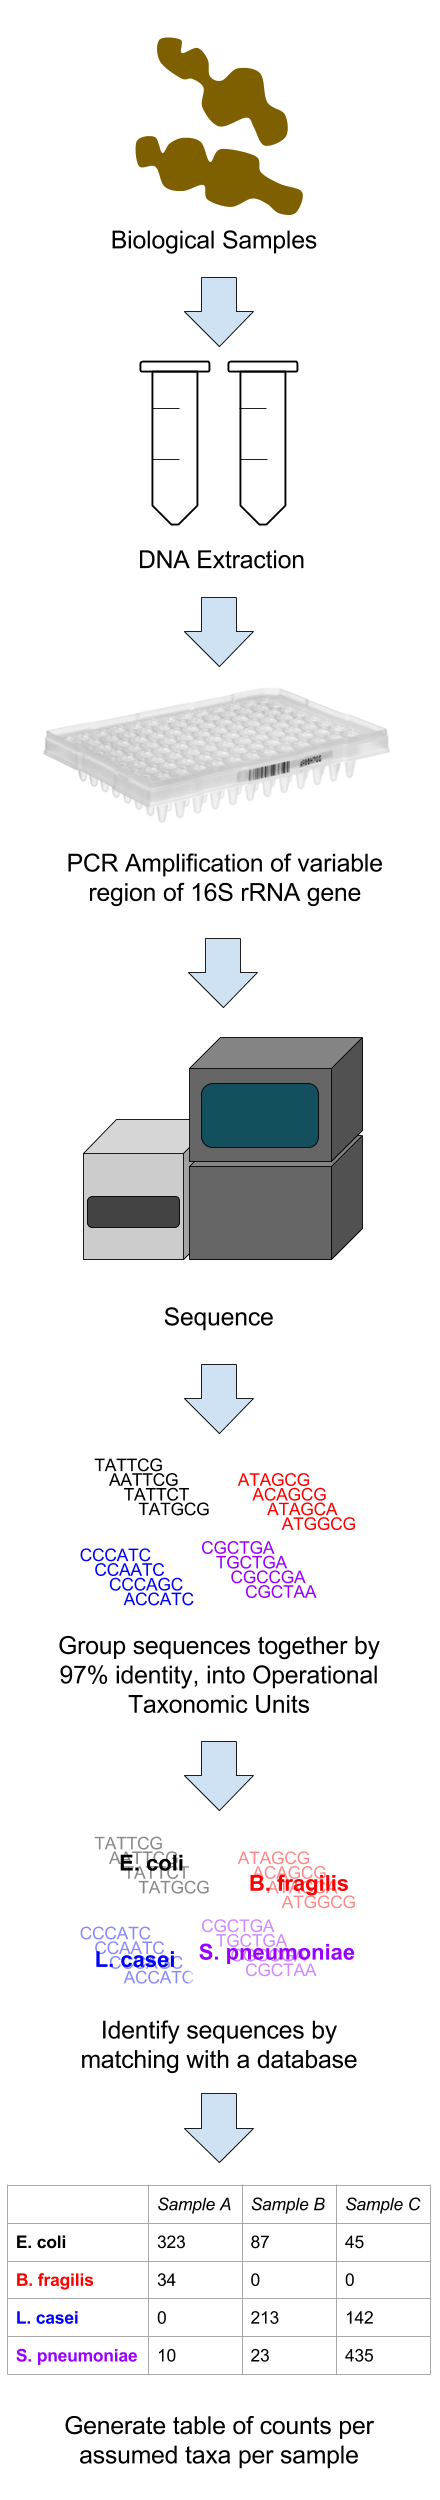
\includegraphics[height=0.8\textheight]{16S_rRNA_pipeline.png}
\caption{A long memory time series\label{ts1}}
\end{center}
\end{figure}

\begin{enumerate}
\item Take a biological sample and extract the DNA
The sample can be collected swabbing the target body site or by collecting samples in some other way. DNA extraction is usually done with common commercial kits.

\item Run a PCR amplification
As discussed previously, the gene tag experiments in this thesis amplify the V4 region of the 16S rRNA gene, following the Earth Microbiome Project protocol (Caporaso, 2012). The set of primers that we use are barcoded, so that we can sequence all the samples in the same sequencing run and differentiate them afterwards.

\item Run sequencing
We use 150 nucleotide paired-end sequencing on the Illumina MiSeq platform. The 150 nucleotide paired ends allow us to overlap paired sequences in the middle to reconstitute the full sequence of the variable region.
\end{enumerate}

\paragraph{Post-sequencing processing}\mbox{}\\
Here are the steps for going from raw sequenced reads to a table of counts per taxa per sample.
\begin{enumerate}
\item Demultiplex the raw sequence
The barcodes are used to separate the sequences according to what sample they came from.

\item Assemble the paired ends of sequenced DNA
The paired sequences are overlapped in the middle, resulting in the full variable region amplified by the primers.

\item Group the reads into operational taxonomic units (OTUs)
We used the mothur software suite to cluster the reads into groups of 97% identity (Schloss, 2009).

\item Annotate the OTUs with bacterial taxonomy
Annotation was done by  matching our OTUs to the SILVA database (Quast, 2013).
\end{enumerate}

Alternatively, an Individual Sequence Unit (ISU) based approach can be taken, where the individual sequences are preserved even after grouping into OTUs, so that different strains within the same OTU can be analyzed separately (Callahan, 2015).

\FloatBarrier

\subsection{Data analysis}
There are two goals in gene tag data analysis. First, is there any structure in the data (separation, clustering, correlations, differentials, etc.)? Second, what drives the structure in the data?

Separation or clustering can be examined by determining the distance between each sample, and using these distances to plot the samples as points on a graph. The following sections will go over the most commonly used distance metric in microbiome research, called UniFrac, as well as the Principal Components Analysis multidimensional scaling method for plotting the points on a graph. Afterwards the data can be visually or mathematically inspected for separation or clustering.

The technique used for determining if taxa are differentially abundant between groups is the same technique used for determining if gene annotations are differentially abundant between groups in the metagenomic experiment, and has its own section, titled “Compositional data analysis”.

\paragraph{UniFrac}\mbox{}\\
Principal Component Analysis is necessary for multivariate statistics, and It is well known that the Principal Component Analysis cannot be performed on proportions, such as the OTU abundances derived from gene tag sequencing. Instead, a Euclidean distance is required (Anderson, 2003).

In 2005, Lozupone et al introduced the UniFrac distance metric, a measure to calculate the difference between microbiomes that incorporated phylogenetic distance (Lozupone, 2005). The goal of UniFrac was to enable objective comparison between microbiome samples from different conditions. In 2007, Lozupone added a proportional weighting to the original unweighted method (Lozupone, 2007). Since then, papers reporting these metrics have garnered over a thousand citations, and enabled research about everything from how kwashiorkor causes malnutrition (Smith, 2013) to how people can have similar microbiomes to their pet dogs (Song, 2013).  Except for Generalized UniFrac, used to make hybrid unweighted and weighted UniFrac comparisons (Chen, 2012), few advances in the metric have occurred since 2007. 

\paragraph{Unweighted UniFrac}\mbox{}\\

\begin{figure}[h]
\begin{center}
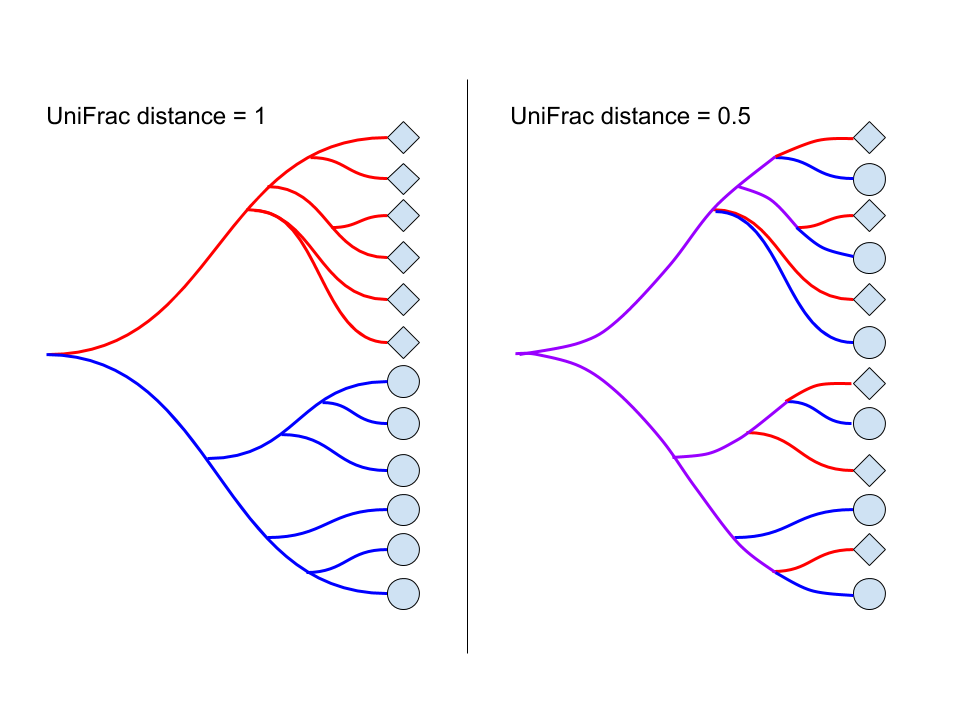
\includegraphics[width=\textwidth]{unifrac.png}
\caption{A long memory time series\label{ts1}}
\end{center}
\end{figure}

Unweighted UniFrac uses an inferred evolutionary distance to measure similarity between samples. It requires a reference phylogenetic tree containing all the taxa present in the samples to be examined. The calculation is performed by dividing the branch lengths shared between the two samples by the branch lengths covered by either sample. A distance of 0 means that the samples have an identical set of taxa detected, and a distance of 1 means that the two samples share no taxa in common.

The qualitative rather than quantitative nature of unweighted UniFrac makes the metric very sensitive to sequencing depth. A greater sequencing depth generally results in the detection of a greater number of taxa. To account for this problem, ecologists use a technique called rarefaction to normalize the sequencing depth across samples by random sampling without replacement (de Cárcer, 2011). However, in unweighted UniFrac samples move relative to the other samples in different rarefaction instances, to the point where they can switch from being a member of one cluster of data to another, as demonstrated in the chapter Expanding the UniFrac Toolbox.

\FloatBarrier

\paragraph{Weighted UniFrac}\mbox{}\\
Weighted UniFrac is an implementation of the Kantorovich-Rubinstein distance in mathematics, also known as the earth mover's distance (Evans, 2012). Rather than looking only at the presence or absence of taxa, each branch length of the phylogenetic tree is weighted by the difference in proportional abundance of the taxa between the two samples. This technique reduces the problem of low abundance taxa being represented as a 0 or by a low count depending on sampling depth. In unweighted UniFrac, such taxa would flip from absent to present, and could skew the measurement: this would be especially problematic if the taxa are on a long branch. In weighted UniFrac, low abundance taxa have a much lower weight and so will have a lower impact on the total distance reported by the metric.

UniFrac is constituted as either a presence/absence (unweighted UniFrac) (Lozupone, 2005), a linear proportion in the form of weighted UniFrac (Lozupone, 2007), or some combination of the two in the form of Generalized UniFrac (Chen, 2012). However, the data are not linear, because the sum of the total number of reads is constrained by the sequencing machinery (Friedman, 2012). Alternative weightings and non-linear transformations of data need to be explored.

\paragraph{Principal Components Analysis}\mbox{}\\
Once the distances between each pair of samples has been calculated, they can be visualized on a plot, with each sample represented as one point. For visualization, the data should be placed so distances are preserved as much as possible, so that clustering and separation of samples can be clearly seen. This is done using the Principal Coordinate Analysis method of multidimensional scaling (Dollhopf, 2001), shortened as PCoA.

To plot all of the samples as points in space such that the distances between each pair of samples are preserved, multiple dimensions are required. In this data specifically, the number of dimensions required is equal to one less than the number of samples. PCoA rescales all the dimensions as components, so that the first component captures the largest variation, or spread of the data, the second component captures the largest variation remaining in the data after the first component, and so on. This way, even if only the first two components are used to plot all the samples as points on a two dimensional graph, the data is spread out to enable visualization of separation or clustering.

After multidimensional scaling the data can be analyzed in several ways. The data can be examined for clustering by k-means analysis (Tibshirani, 2005). The points can also be measured for separation by looking only at their position on the first principal component axis, especially if the first axis covers the majority of the variation in the data set. With each sample associated with a number on the first principal component axis, one can examine the effect size of two different groups by taking the mean positions and dividing by the standard deviation.

\section{The metagenomic experiment}
Deep metagenomic sequencing provides an estimate of the proportion that each type of gene comprises out of the total genes present in the genetic material of the sample. This can be used to answer questions such as:

\textit{What is the metabolic potential of the microbial community?}
The metabolic potential is made up of all the protein functions that are coded by the genetic material present in the sample. Biologically speaking, these protein functions represent the enzymatic reactions that the microbiome could produce if all the genes were expressed. For example, the human gut microbiome has more genes related to methanogenesis, compared to the average sequenced microbe (Gill, 2006).

\textit{Are any genes, functional categories of genes, or metabolic pathways made up of genes differentially abundant between groups?}
In 2006, Turnbaugh et al published a paper showing that an obesity associated gut microbiome in mice had an increased capacity for energy harvest (Turnbaugh, 2006), sparking more research into the gut microbiome and obesity related ailments such as diabetes (Larsen, 2010) and non-alcoholic fatty liver disease (Zhu, 2013). The ability to check if genes, functional categories of genes, or pathways are differentially abundant between groups allows scientists to find clues about the mechanisms by which the microbiome affects certain diseases.

All of this information can be determined by either imputation or actual sequencing, discussed in the next sections.

\subsection{Sequencing}

\begin{figure}[h]
\begin{center}
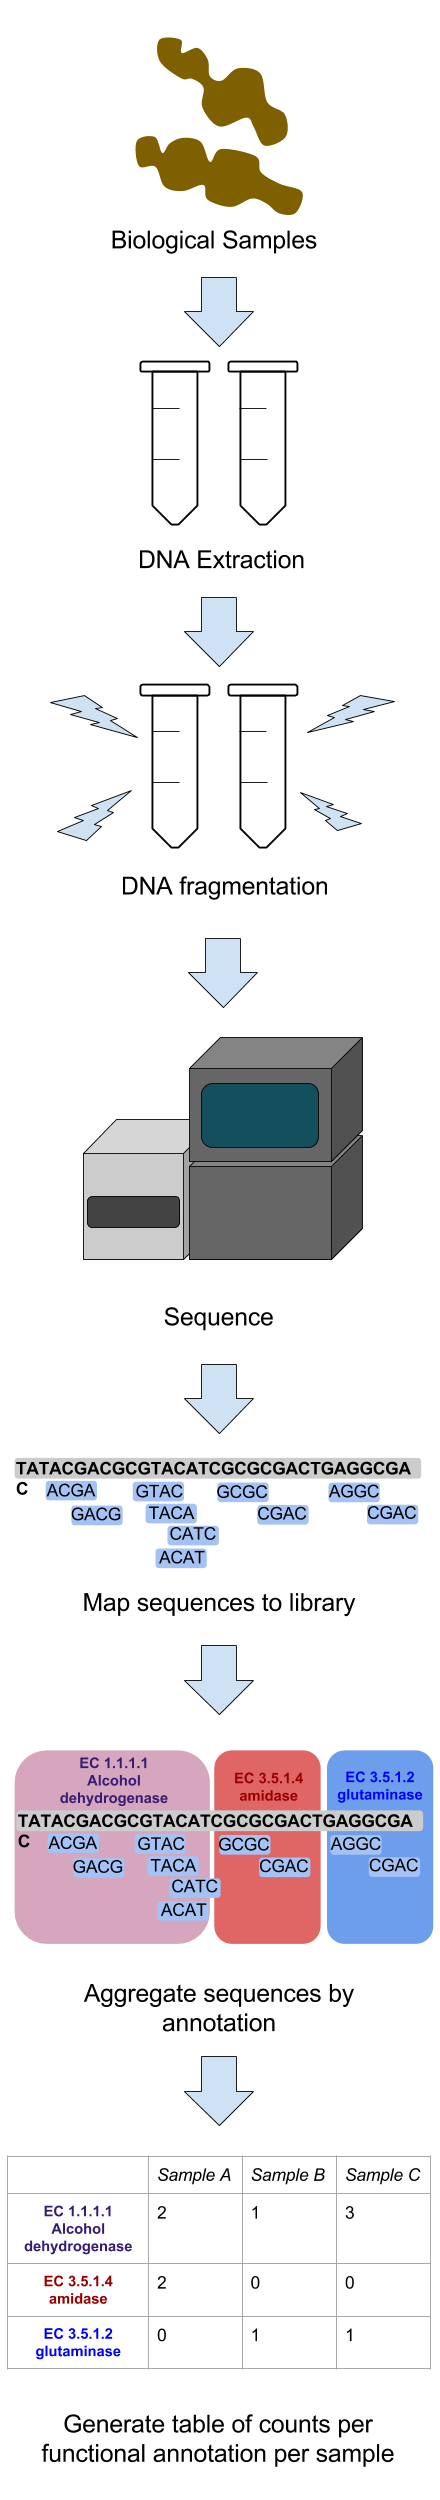
\includegraphics[height=0.8\textheight]{Metagenomic_pipeline.png}
\caption{A long memory time series\label{ts1}}
\end{center}
\end{figure}

The goal of metagenomic analysis is to examine the metabolic potential of the microbiota in the microbiome. This is done by identifying genes, sorting them by the known function of the protein for which they code (such as the catalyzation of a certain reaction), and checking if any functions are differentially present between conditions. Further analysis can also include checking for pathway enrichment, and assembling the sequenced reads into genomes. The general protocol for metagenomic analysis is as follows:

\begin{enumerate}
\item Take a biological sample and perform DNA extraction
The sample can be collected by swabbing the target body site or collecting excretions.

\item Prepare the DNA for sequencing
Fragment the DNA, and filter for the desired size. These steps are all part of the standard Illumina library prep protocol for the HiSeq. There are two options for fragment size, either 50 or 100 nucleotides in length, and we chose the longer one for easier assembly and mapping.

\item Sequence the DNA.
We performed single end sequencing on the Illumina HiSeq platform, with our samples barcoded so that they could be pooled into the same sequencing run.

\item Create an annotated library of reference sequences
The annotated library contains annotations about what kind of protein each sequence codes for. The first step to creating the annotated library is to gather a database of sequences. The database of sequences can be created before the sequencing is complete by gathering all the genomes of all the bacterial strains predicted to be present in the sample, or it can be created after sequencing by assembling the sequenced reads into parts of genomes. The second step is to annotate the sequences with predicted protein functions. Some publically available genomes already have protein annotations. For genomes or partial genomes without annotations, the placement of genes can be predicted by looking for open reading frames, and these predicted genes can be aligned with databases such as SEED (Overbeek, 2005) or KEGG (Kanehisa, 2000) to match them with functional annotations, using the BLAST algorithm (Altschul, 1990).

\item Map the sequenced reads to the library.
Mapping is the process of annotating the sequenced reads by aligning them with sequence that has already been annotated. We used Bowtie2 (Langmead, 2012) to map our sequenced reads to the annotated library created in the previous step. Bowtie2 aligns similar sequences together.

\item Determine how many mapped reads match each functional annotation.
Once the sequenced reads have been mapped to the annotated reference sequence, the number of reads sequenced for each annotation can be counted up. The end result is a table of counts per gene annotation per sample.
\end{enumerate}

Issues with sequencing and the analysis of sequencing data arise from sampling and the fat nature of the data. The sequences that are read by the sequencer are only a small fraction of the DNA from the sample. Additionally, primers used for sequencing may be biased for certain sequences more than others. Lastly, the data is very fat, which is to say that there are magnitudes more variables (in the form of functional annotations of genes) than there are samples. This makes it difficult to have enough power to detect small differences in the data, a concept expanded upon in the Points of Failure section below.

\FloatBarrier

\subsection{Imputation}
Deep metagenomic sequencing can be imputed using a tool called PiCrust from a gene tag experiment (Langille, 2013). PiCrust uses the Greengenes database (DeSantis, 2006) to identify the bacterial taxa in the sample, and pulls their genomes from the Integrated Microbial Genomes database (Markowitz, 2012). With the genomes, the program tries to predict what would be seen if the samples underwent deep metagenomic sequencing. For taxa without a fully sequenced genome, PiCrust infers the genetic content based on ancestors in the phylogenetic tree. PiCrust produces metagenome predictions with Spearman r=~0.7 (Langille, 2013), compared to a full metagenomic sequencing experiment.

Imputation is useful for identifying potential correlations that should be explored and validated further, but should not be used to make conclusions. The issues with imputation include all the issues with sequencing, plus the added variation in its imperfect correlation.

\subsection{Data analysis}
Data analysis can be performed by performed by seeing if functions are differentially abundant between samples in different groups (described in the “Compositional data analysis” section), examining functional categorizations, and checking for pathway enrichment.

\paragraph{Functional categorization}\mbox{}\\

\begin{figure}[h]
\begin{center}
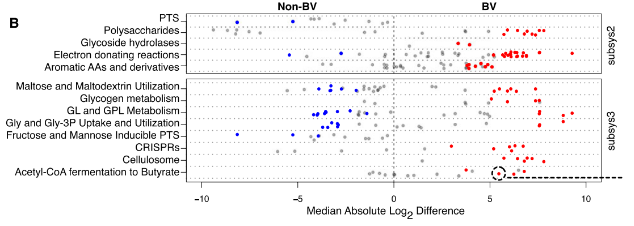
\includegraphics[width=\textwidth]{stripchart.png}
\caption{A long memory time series\label{ts1}}
\end{center}
\end{figure}

We use the SEED annotation, which has four different levels of categorization. Subsystem 4 is the most atomic categorization level and describes the specific function of the protein group, for example, “Isovaleryl-CoA dehydrogenase (EC 1.3.99.10)”. Subsystem 3, 2, and 1 are increasing more general levels of categorizations, from enzyme families to large categorizations such as genes related to carbohydrate metabolism.

Even if the subsystem 4 functional categories are not significantly different between groups, they each have an effect size with a direction. Stripcharts can be used to plot the effect sizes of the subsystem 4 categories for a larger category. For example, by plotting the effect sizes of all the subsystem 4 categorizations under Carbohydrate Metabolism, one can visually see if there are any obvious directional trends for carbohydrate metabolism functions being more present in the experimental group compared to the control.

\FloatBarrier

\paragraph{Pathway enrichment}\mbox{}\\
Biological pathways can be thought of as made up of a series of chemical reactions, each catalyzed by a protein enzyme, which is encoded by a gene. KEGG (Kyoto Encyclopaedia of Genes and Genomes) is a manually curated annotation database that matches genes to pathways (Kanehisa, 2000). This database allows researchers to see if there is differential abundance of pathways encoded by functionally annotated genes, even when the genes may not be differentially abundant by themselves.

\section{Points of failure}
The Huttenhower lab has organized the Microbiome Quality Control project (MBQC) at http://www.mbqc.org/. Preliminary results show that despite being given the same samples, different participating labs can come up with vastly different results. This lack of reproducibility is caused by a lack of consensus on the correct way to analyze microbiome data. The following sections explore different aspects of microbiome data that contribute to this.

\subsection{Collection methods differ}
These experiments are very sensitive to batch effects because microbiome composition can be very variable within groups such that the effect size of a difference between groups can be small. Wherever possible, all samples should be processed in the same batch. Analysis should also be done to check if samples extracted on different dates or sequenced with different primers separate into clusters, to make sure that there is no systematic bias in the data.

\subsection{Microbiome data is highly variable between individuals}
One highly studied body site is the gut, and the gut microbiome can be affected very strongly by diet (Turnbaugh, 2009). This among other factors lead to a highly diverse gut microbiome between subjects for reasons unrelated to the disease being studied, creating a lot of noise, potentially obscuring real effects or even creating the appearance of false effects.

Generally experiments of this nature typically have low sample sizes due to budget constraints, sample collection difficulties, patient compliance, and other issues. To increase cost effectiveness and reduce batch effects, we run all the samples in an experiment on the same sequencing run, by means of a primer design (Gloor 2010).

There are several models for computationally analyzing the variance within conditions in order to determine if operational taxonomic units are significantly differentially abundant, most of which were originally desigend for RNA-seq experiments on single organisms (Pachter, 2011). Currently the most popular tools for analyzing differential abundance are EdgeR (Robinson, 2010), DESeq2 (Love, 2014), and MetagenomeSeq (Paulson, 2014). EdgeR was cited by 1,130 papers in 2015 according to Google Scholar. DESeq2 and MetagenomeSeq are part of the QIIME pipeline, which was cited by 1,620 papers in 2015.

EdgeR and DESeq2 use the negative binomial distribution. The negative binomial distribution allows the variance of data to be estimated given the mean, through a function. The function is determined by collecting the mean and variance for all the counts for each OTU in each experimental condition, and fitting the variances according to the negative binomial distribution. This vastly underestimates the variance at low counts, which represent the sampling of low abundance OTUs, and can be very different between replicates. Underestimating the variance at low counts produces spurious low p-values for low count OTUs (Fernandes, 2013).

MetagenomeSeq uses the Zero-Inflated Gaussian (ZIG) model, which is a binomial distribution of counts (that may include zero counts), plus a function to predict how many extra zeros there will be. This doesn’t work well when the total number of reads are not well matched, because then there will be much more zeros in the data set with less reads, due to having a lower sequencing depth, and a consistent total read count is required between samples according to page 2 of the supplementary material in the first metagenomeSeq paper (Paulson, 2013).

For my differential abundance analysis, I’ve used ALDEx2, which samples from the Dirichlet distribution to model variation in the data (Fernandes, 2014). After a number of samples, the mean value and mean variance are used to determine if OTUs are differentially abundant between groups, an approach that is believed to result in greater sensitivity and equivalent specificity compared to the DESeq2 approach (Fernandes, 2014).

\subsection{Microbiome data involves the comparison of many features}
Oftentimes, the number of taxa or gene functions comparisons is a magnitude larger than the sample size. This is known in statistics as having more variables than observations, or having fat data. The higher the ratio of variables to observations are, the less likely the principal components analysis is to be reliable (Osborne, 2004).

Researchers should include multiple test corrections to ensure that the results they are reporting are true, at the expense of having p-values less than 0.05. Unfortunately many studies have been published in high impact journals without multiple test corrections, including a famous paper linking the gut microbiome to autism published in Cell (Hsiao, 2013).

\subsection{Microbiome data is compositional}
There are several core truths about microbiome data that should be considered when making an analysis strategy.

First, the total number of reads per sample is irrelevant to the biological implications of the data, as it is limited by how the samples were processed and the sequencing platform. Based on spurious correlations discovered in organ size research, it is known that given compositional data (such as bone lengths as a proportion of height, or OTU abundances that add up to the total number of counts per sample), analysis with the assumption that the variables (bone lengths or OTU counts) are independent lead to spurious positive correlations (Pearson, 1896). The variables thought to be independent are related by the sum they are divided by. Additionally, the constrained sum causes the abundance of different taxa to appear to be negatively correlated with each other when analyzed by conventional statistics. When one taxa increases in abundance, the counts detected in other taxa decrease in abundance, even if the taxa are not decreasing in abundance biologically.

Second, removing an entire variable (an OTU in gene tag sequencing, or a functional annotation in deep metagenomic sequencing) from the analysis should not change correlations between OTUs. Removing variables occur routinely in microbiome research, such as when rare OTUs are discarded. Without a data transformation, removing variables will change the correlation between variables (Aitchison, 1986).

To ensure that these conditions are met, data should be analyzed in a compositional way. Several types of log ratio data transformations are recommended to allow the data to be analyzed by standard Euclidean methods (Aitchison, 1986). The type that makes the most sense for microbiome data is the centered log ratio transform. The centered log ratio transform is performed by dividing each proportional abundance by the geometric mean of all the proportional abundances, and taking the logarithm. The geometric mean acts as a low level baseline abundance in microbiome data. Taking the logarithm of the ratio allows for a consistent measurement whether the large number is in the numerator or denominator of the ratio.

The centered log ratio transform prevents the total number of reads from affecting the measurement, so long as the geometric mean is a stable baseline, a condition met in a typical microbiome data set [CITATION NEEDED]. The centered log ratio transform also allows for coherent subcompositional data analysis as remaining values are not affected when entire variables are removed.

Compositional techniques such as those espoused in the Analysis of Composition of Microbiomes (ANCOM) framework (Mandal, 2015) and the ANOVA-Like Differential Expression 2 (ALDEx2) software (Fernandes, 2014) should be used to prevent spurious correlations and promote consistent data analysis. However, these techniques are not yet mainstream in the field.

\subsection{Microbiome data is sparse}
One of the fundamental challenges in analyzing differential abundance is accounting for zeroes. Unlike a presence/absence test, a zero does not necessarily mean that the expression is not there. The expression could be present in an amount smaller than the resolution of the test. This is a problem because when statistical methods are used to examine significantly different expression, the comparison of zero values to non-zero values are likely to come out as significant whether or not the expression is differential. Additionally, the log transformations used in compositional data analysis cannot be performed on zeros.

Two methods have been suggested in the literature to account for zeros. The first is simply to add a small arbitrary value to each zero, as suggested in the original literature about the statistical analysis of compositional data (Aitchison, 1986). This is used in ALDEx2, and the arbitrary value is chosen to be 0.5, representing complete uncertainty in whether or not a zero count in one sample (where the OTU or gene has non zero counts in other samples) would be a 0 or a 1 in a technical replicate (Fernandes, 2013).

The second method is to take a Bayesian approach where the likelihood that a zero could be changed to a positive count if the sample were resequenced is estimated, based on . This is implemented by the cmultRepl command in the zCompositions package in R (Palarea-Albaladejo, 2015). Based on the shape of the rest of the data for the same sample, the average value of the count detected if a zero were resequenced is determined, and the zeros are all replaced by this fraction.

The microbiome field is quite new, and has been undergoing many exciting developments. Gold standards must be set to ensure that studies are replicable, and that published research represents the biological reality.

\section{The gut microbiome in atherosclerosis-susceptible and atherosclerosis-resistant patients}

\section{The gut microbiome in patients with non-alcoholic steatohepatitis compared to healthy controls}












Here is a picture of a long memory time series. 
\begin{figure}[ht]
\begin{center}

\includegraphics[height = 9cm, width = 9cm]{pic1.jpeg}
\caption{A long memory time series\label{ts1}}
\end{center}
\end{figure}

Here's a table.
\begin{table}[ht]
\begin{center}
\begin{tabular}[ht]{|c|lr|c|} 
%c stands for centre, l for left, r for right; the | puts lines in between, and the hline puts a horizontal line in
\hline
$n$ & $\alpha$ &$n\alpha$ & $\beta$\\
\hline
1 & 0.2 & 0.2 & 5\\
\hline
2 & 0.3 & 0.6 & 4\\
\hline
3 & 0.7 & 2.1 & 3\\
\hline
\end{tabular}
\caption{A random table \label{tab1}}
\end{center}
\end{table}

\begin{eqnarray}
y &=& mx + b \label{eq1}\\
&=& ax+ c
\label{eq2}
\end{eqnarray}

This is an un-numbered equation, along with a numbered one. 
\begin{eqnarray}
u &=& px \nonumber\\
p &=& P(X=x) \label{eqn3}
\end{eqnarray}

Look at Table \ref{tab1} and Figure \ref{ts1} and equations \ref{eq1},  \ref{eq2}, and \ref{eqn3}.

Let's do some matrix algebra now.

\begin{equation}
det\left(\left|\begin{array}{ccc} 2 & 3 & 5\\
4 & 4 & 6\\
9 & 8 & 1
\end{array}\right|\right) = 42
\end{equation}

In the equation and eqnarray environments, you don't need to have the dollar sign to enter math mode.

\begin{eqnarray}
\alpha = \beta_1 \Gamma^{-1}
\end{eqnarray}

This is citing a reference ~\cite{mygood11111}.  This is citing another ~\cite{mrx05}.  Nobody said something ~\cite{Nobody06}.

\chapter{Expanding the UniFrac toolbox}
\include{unifrac_paper/expanding_the_unifrac_toolbox}
\chapter{The human microbiome and non-alcoholic fatty liver disease}

\section{Introduction}
Non alcoholic fatty liver disease (NAFLD) has been on the rise along with obesity, affecting a fifth to a third of the North American population \cite{preiss2008non}. Most people with NAFLD remain asymptomatic, however, in up to a third of patients NAFLD can progress to non-alcoholic steatohepatitis (NASH), causing inflammation and scarring in the liver, and decreasing the 5 year survival rate to 67\% \cite{propst1995prognosis}. If we can shed some light on the process by which people progress from NAFLD to NASH, we might be able to find treatments to prevent NASH.

There are several known genetic factors that increase the risk of progression to NASH. The I148M variant of the Patatin-Like Phospholipase Domain Containing 3 gene (PNPLA3) correlates with a 3.2 fold increased risk of NASH from NAFLD when present homozygously, compared to to patients without the variant \cite{sookoian2011meta}. Additionally, mice with a toll-like receptor 4 knockout had lower lipid and injury accumulation markers when fed a methionine/choline-deficient diet which would normally induce steatohepatitis in wild type mice \cite{rivera2007toll}.

On the epigenetic level, genes are differentially methylated in advanced NAFLD compared to mild NAFLD. 11\% of genes are differentially hypomethylated in advanced NAFLD (compared to 3\% hypermethylated), leading to increased expression \cite{murphy2013relationship}. On a hormonal level, estrogen has been shown to inhibit fibrosis in rats \cite{yasuda1999suppressive}. On a metabolite level, Raman et al. found differences in the number of volatile organic compounds detected in patients with NAFLD compared to obese patients without NAFLD \cite{raman2013fecal}. Reactive oxygen species have also been implicated in NASH due to their involvement in the mechanism of steatohepatitis-inducing drugs \cite{berson1998steatohepatitis}.

A 2001 paper performed C-D-xylose-lactulose breath tests and measured tumor necrosis factor alpha levels to determine presence of bacterial overgrowth, and found increased bacterial overgrowth in 22 patients with NASH compared to 23 healthy controls \cite{wigg2001role}. Some papers claim a link between ethanol-producing gut bacteria and NAFLD \cite{zhu2013characterization} \cite{jiang2015dysbiosis}, however, no multiple test correction was performed in these studies.

Several papers have already been published in the literature on the topic of NAFLD and the gut microbiome:

\begin{figure}[h]
\begin{center}
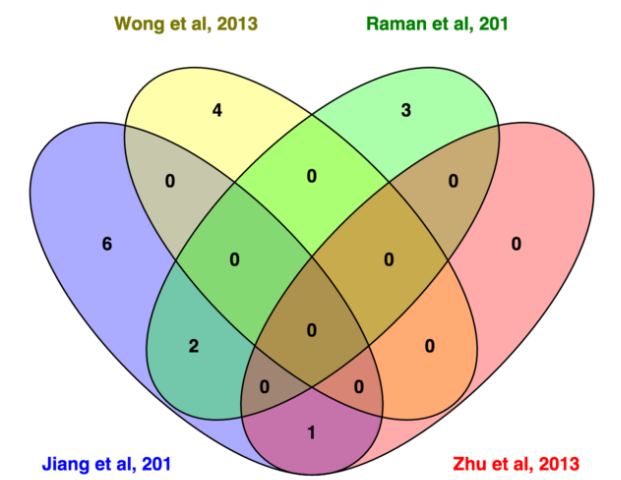
\includegraphics[width=0.7\textwidth]{nafld_papers.png}
\caption{\textbf{Venn diagram of genus found to be differentially abundant by different studies between NASH/NAFLD and healthy controls.} Boursier et al 2015 is not included as they reported a p-value of less than 0.05 for the Bacteroides genus only, which was not reported in any of the other studies. Only 3 out of the 16 genus claimed to be differentially abundant were the same in two studies: Escherichia was found in the Zhu \cite{zhu2013characterization} and Jiang \cite{jiang2015dysbiosis} studies, and Lactobacillus and Oscillibacter were found in the Jiang \cite{jiang2015dysbiosis} and Raman \cite{raman2013fecal} studies.}
\end{center}
\label{nafld_fig1}
\end{figure}

\begin{itemize}
\item Jiang et al, 2015 \cite{jiang2015dysbiosis} compared 53 NAFLD patients with 32 healthy controls

\item Zhu et al, 2013 \cite{zhu2013characterization} compared 16 non-obese controls, 25 obese patients, and 22 NASH patients

\item Raman et al, 2013 \cite{raman2013fecal} compared 30 NAFLD patients with 30 healthy controls

\item Wong et al, 2013 \cite{wong2013molecular} compared 16 NASH patients with 22 healthy controls

\item Boursier et al, 2015 \cite{boursier2016severity} compared 30 patients with F0 or F1 fibrosis to 27 patients with F2 or greater fibrosis, 35 of which had NASH
\end{itemize}

Of these, only Raman et al \cite{raman2013fecal} reported using a multiple test correction.

These five studies do not form a consistent story about the gut microbiome and NAFLD. We hope to run our own analysis rigorously, such that our results are replicable. Additionally, we are running a deeply sequenced metagenomic study, which hasn’t been done in the past.

\FloatBarrier

\section{Methods}
In total, 92 samples were collected: 41 from patients with NASH, 18 from patients with SS, and 33 from healthy controls.

[TO DO: include information about sample collection and exclusion criteria]

DNA extraction was performed with the \href{http://omegabiotek.com/store/product/stool-dna-kit/}{E.Z.N.A.® Stool DNA Kit}, and the protocol was followed with the addition of lysozyme with an extra 30 minute incubation at 37 degrees Celcius, between steps 2 and 3.

\subsection{16S rRNA gene tag experiment}

DNA was amplified by PCR according to the Earth Microbiome protocol \cite{caporaso2012ultra}, with the addition of barcodes so that all the samples could be sequenced in the same sequencing run \cite{gloor2010microbiome}. The DNA was sequenced on the Illumina MiSeq platform with paired end 150 nucleotide reads, producing 34955148 reads in total.

Reads were overlapped with Pandaseq \cite{masella2012pandaseq}, clustered into Operational Taxonomic Units using UCLUST \cite{edgar2010search}, and annotated with the SILVA database \cite{quast2013silva}, producing a table of counts per operational taxonomic unit per sample. 16809756 reads (48\%) were succesfully overlapped and annotated with 232 OTUs. Differential abudance was analyzed using ALDEx2 \cite{fernandes2014unifying}.

\subsection{Metagenomic experiment}

A deep metagenomic sequencing experiment was performed using samples from 10 healthy controls and 10 of the patients with NASH. Samples from healthy patients were selected to exclude confounding factors, such as having a different country of birth, which could affect diet. Samples from NASH patients were selected for the strongest NASH phenotype.

The DNA was sequenced on the Illumini HiSeq platform, with single end 100 nucleotide reads. Samples were barcoded and sequenced on the same sequencing run. After sequencing, the reads were quality filtered and demultiplexed to separate the reads for each sample, yielding 1914714572 reads in total.

To annotate the reads, we used a two pronged strategy:

First, we created a reference library using the inferred taxa from the 16S rRNA gene tag experiment. For each genus the OTUs were annotated with, we randomly picked 10 strain genomes from the NCBI bacterial genome database. For genus where there were less than 10 fully sequenced representatives, we selected all genomes available. The library was made with 1134 genomes from 104 bacterial genus. The library was then clustered at 99\% identity for each genus using CD-HIT \cite{li2006cd} to decrease the number of sequences in the library from 3495887 to 2256844. Annotation was performed with the SEED database \cite{overbeek2005subsystems}, and sequenced reads were mapped onto this library. Out of 1914714572 reads total, 585382507 (30.6\%) were annotated by this method, over 5836 unique SEED hierarchy annotations. The code for the \href{https://github.com/ruthgrace/make_functional_mapping_library}{reference library creation} and \href{https://github.com/ruthgrace/mapping_library_annotated_counts}{annotation} is on GitHub.

Second, we assembled the reads per sample de novo using Trinity \cite{haas2013novo}, producing 8847816 sequences, and removed sequences that matched our reference library with 90\% identity as determined by BLAST \cite{altschul1990basic}, leaving 5876423 sequences. [FILL IN THIS] of these assembled sequences were successfully annotated with the SEED database \cite{overbeek2005subsystems}, and sequenced reads were mapped onto this. [FILL IN THIS] additional reads were annotated by this method, over [FILL IN THIS] unique SEED hierarchy annotations. The code for the custom assembly pipeline is on \href{https://github.com/ruthgrace/exploring_nafld_assembly}{GitHub}. The data from both prongs was amalgamated into a single table of counts per annotation per sample.

Differential abudance was analyzed using ALDEx2 \cite{fernandes2014unifying}.

\subsection{MetaPhlAn}

MetaPhlAn (Metagenomic Phylogenetic Analysis) \cite{segata2012metagenomic} is a piece of software that allows one to infer the taxa present based on the metagenomic sequencing experiment. We used this to generate a count table per taxa per sample, and will compare it to our experimental results from the 16S rRNA gene tag sequencing experiment.

\section{Results}

\subsection{16S rRNA gene tag experiment}
The top five genus detected by 16S rRNA gene sequencing (excluding unclassified bacteria) were: Incertae_Sedis, Bacteroides, Faecalibacterium, Blautia, and Pseudobutyrivibrio (Fig.~\ref{nafld_16s_barplot}).

\begin{figure}[h]
\begin{center}
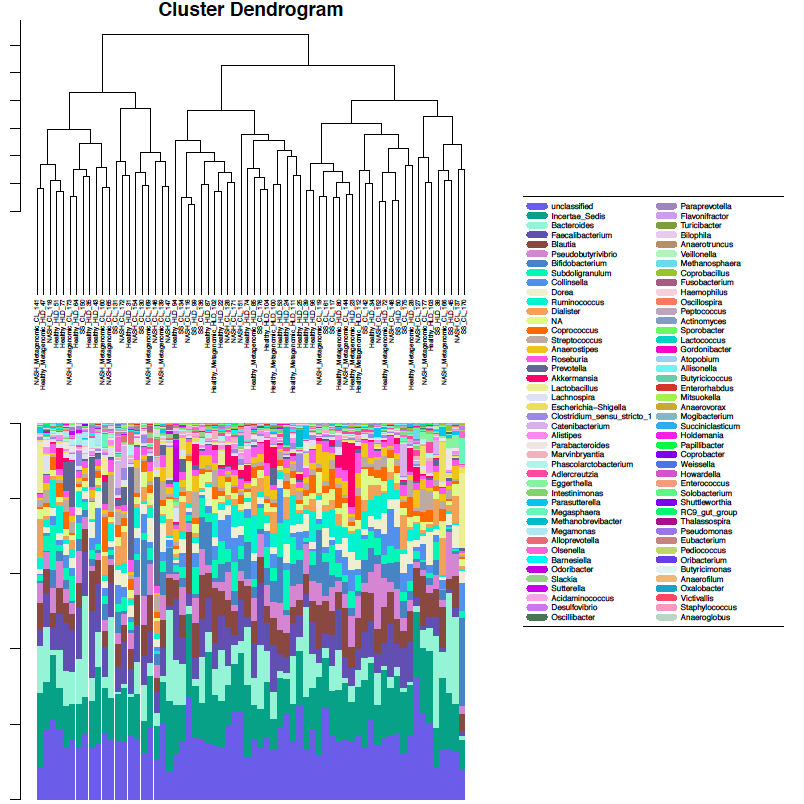
\includegraphics[width=0.95\textwidth]{16s_genus_barplot.png}
\caption{\textbf{16S rRNA gene tag sequencing per sample bar plot.} Each column of this bar plot represents one sample, and each color represents one bacterial genus. Genus are listed in the legend in order of decreasing total abundance across all samples. Samples do not cluster according to their condition (healthy, simple steatosis, or nonalcoholic steatohepatitis).}
\end{center}
\label{nafld_16s_barplot}
\end{figure}

No obvious structure or separation is evident from the principal components analysis in Fig.~\ref{nafld_fig2}. Furthermore the variance explained by each principal component axis is not notably high, indicating a rather uniform data set.

\begin{figure}[h]
\begin{center}
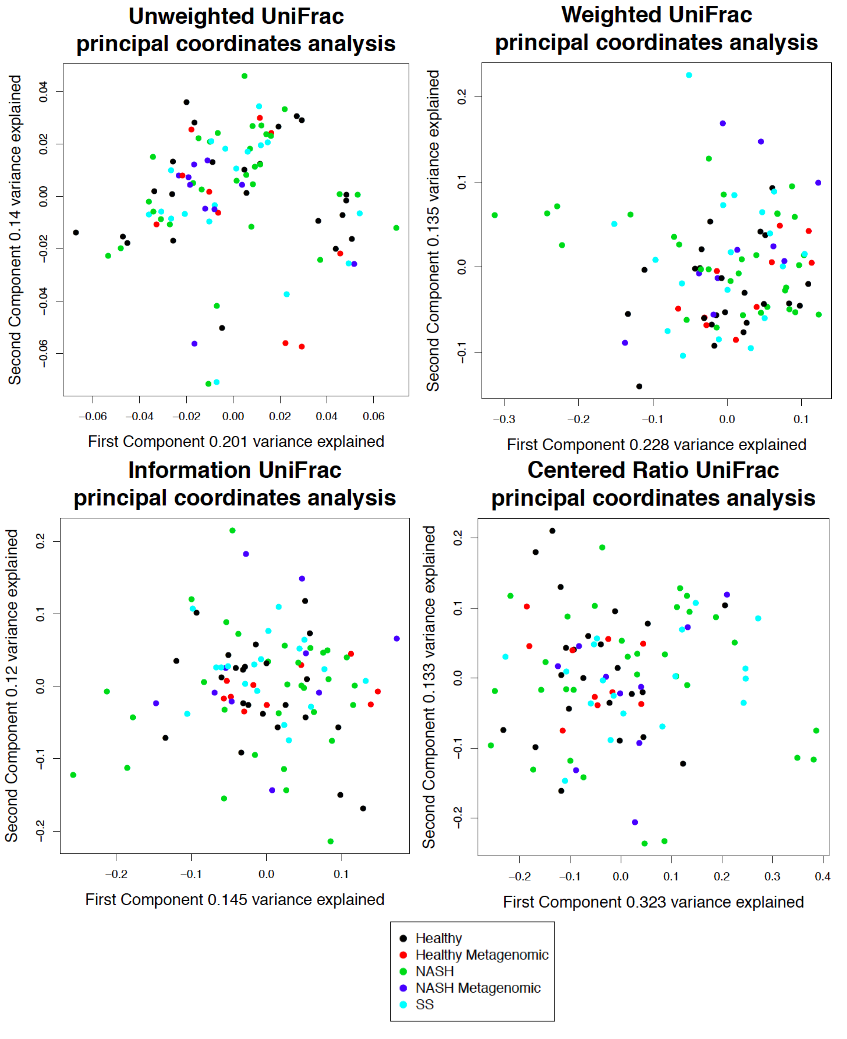
\includegraphics[width=0.95\textwidth]{nafld_16s_pcoa.png}
\caption{\textbf{Principal Components Analysis of 16S rRNA gene tag sequencing data with different UniFrac weightings.} Each point represents one sample, and the distances between the samples have been calculated using different UniFrac metrics, taking into account phylogenetic as well as abundance information. There is no obvious separation between groups by any of the UniFrac weightings. Furthermore the variance explained by each principal component axis is not notably high, indicating a rather uniform data set.}
\end{center}
\label{nafld_fig2}
\end{figure}

\begin{figure}[h]
\begin{center}
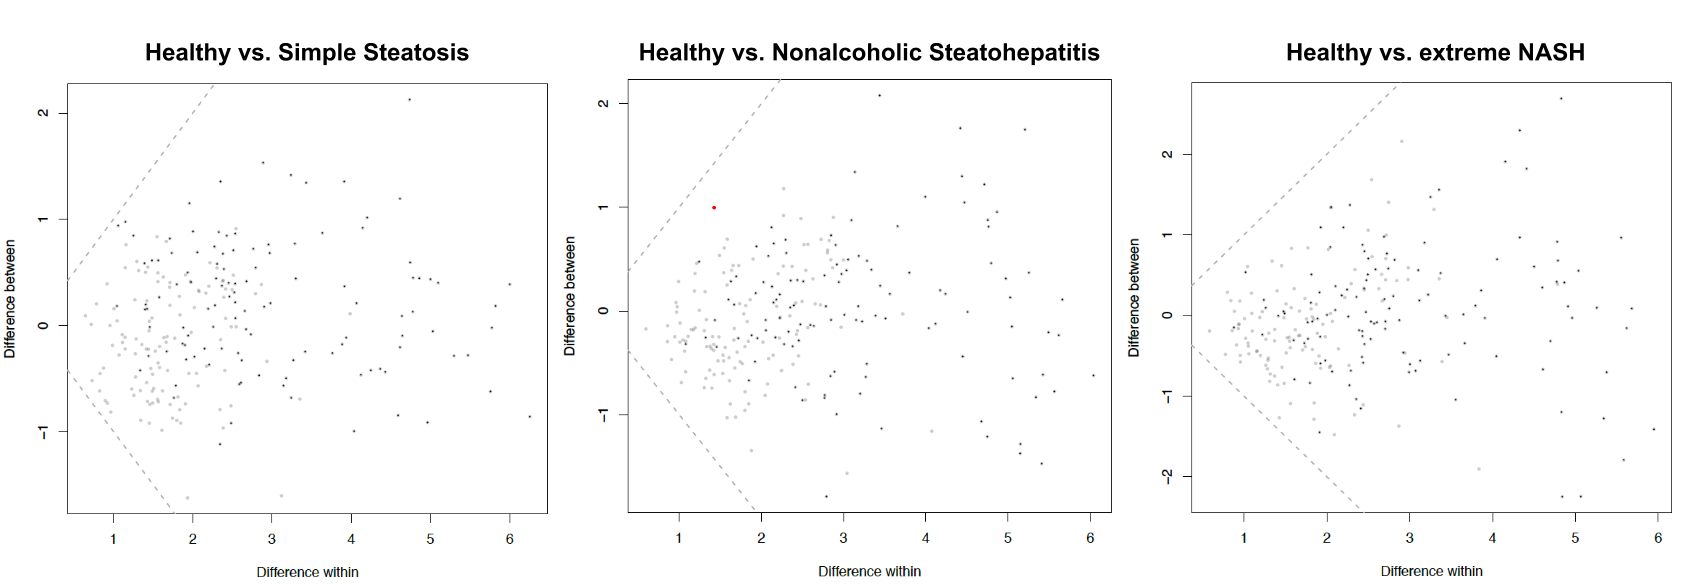
\includegraphics[width=0.95\textwidth]{nafld_16s_aldex.png}
\caption{\textbf{Difference within vs. difference between groups.} Each point represents one OTU, and the differential abundance of that OTU within groups is plotted against the differential abundance between groups. None of the OTUs are more different between groups than within groups. The healthy samples used for these comparisons are the 10 healthy samples used for the metagenomic study. The extreme NASH samples used for these comparisons are the subset of the NASH patients selected for the metegenomic study.}
\end{center}
\label{nafld_fig3}
\end{figure}

\begin{figure}[h]
\begin{center}
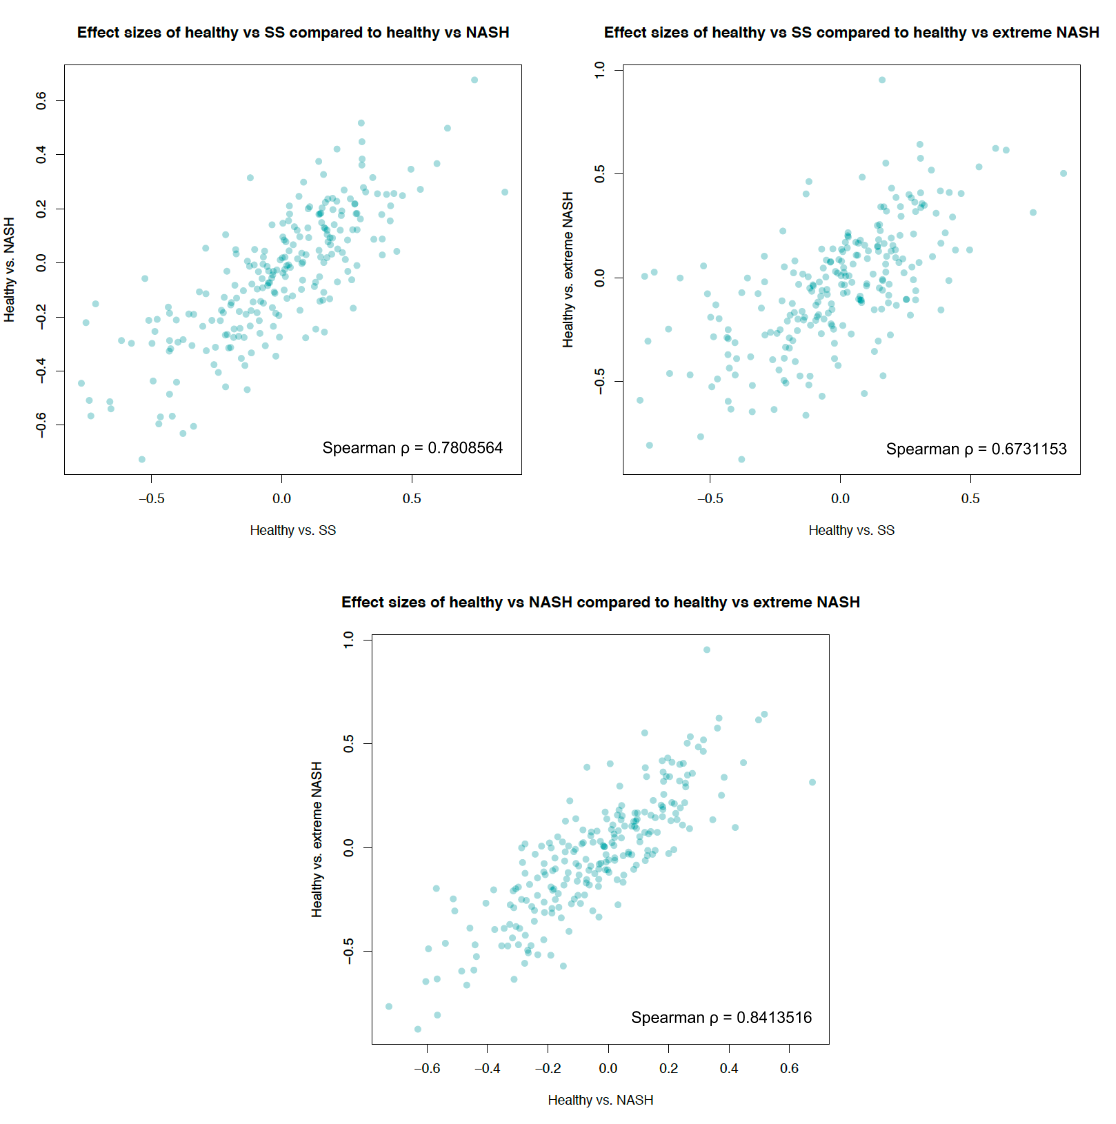
\includegraphics[width=0.95\textwidth]{nafld_16s_effect_sizes.png}
\caption{\textbf{Correlation in effect sizes of different group experiments.} Each point represents one OTU, and the effect size of that OTU in one comparison (for example, comparing the gut microbiome of healthy patients with patients who have simple steatosis) is plotted against the effect size of that OTU in another comparison. The healthy samples used for these comparisons are the 10 healthy samples used for the metagenomic study. The extreme NASH samples used for these comparisons are the subset of the NASH patients selected for the metegenomic study. The y intercepts of the regression lines are all between 0.005 and 0.025, close to zero. The median difference in the absolute effect sizes is -0.02076 for Healthy vs. NASH - Healthy vs. SS, 0.017070 for Healthy vs. extreme NASH - Healthy vs. SS, and 0.04256 for Healthy vs. extreme NASH - Healthy vs. NASH.}
\end{center}
\label{nafld_fig4}
\end{figure}

A differential expression analysis performed with ALDEx2 yielded no significantly differentially abundant OTUs (Fig.~\ref{nafld_fig3}). However, the effect size of each OTU in each comparison is correlated, and the regression line indicates that the effect sizes are higher in the Healthy vs. extreme NASH compared to the Healthy vs. SS or Healthy vs. NASH comparison.

\subsection{Metagenomic experiment}

\paragraph{MetaPhlAn}\mbox{}\\

We ran the metagenomic sequences through MetaPhlAn to infer what the results would be with 16S rRNA gene tag sequencing, so that we could compare with our empirical 16S rRNA gene tag sequencing results. The effect size Spearman coefficient (Fig.~\ref{nafld_metaphlan_effect}) is smaller than the effect size coefficient between the healthy vs. SS and healthy vs. NASH comparison, even though in this case the same samples are being compared.

\begin{figure}[h]
\begin{center}
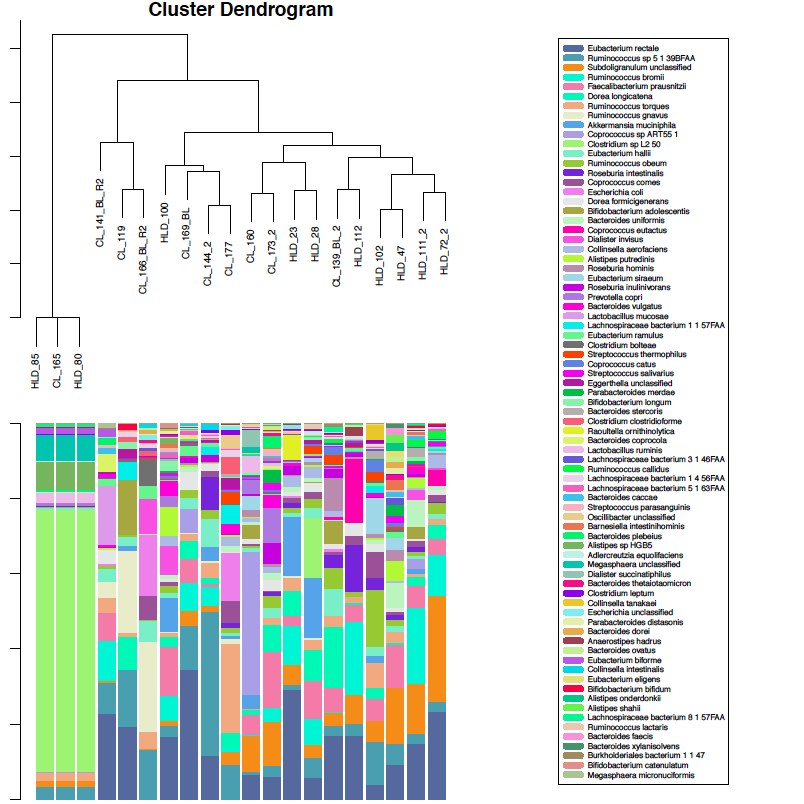
\includegraphics[width=0.95\textwidth]{metaphlan_barplot_dendogram.png}
\caption{\textbf{Taxa barplot dendogram derived from MetaPhlAn.} The metagenomic reads were input into MetaPhlAn to generate a count table. The taxa in the count table were filtered such that only taxa with at least 1\% abundance in any sample was kept. Note that three samples were output to have exactly the same counts (HLD_80, HLD_85, and CL_165), despite not all being in the same condition.}
\end{center}
\label{nafld_metaphlan_barplot}
\end{figure}

\begin{figure}[h]
\begin{center}
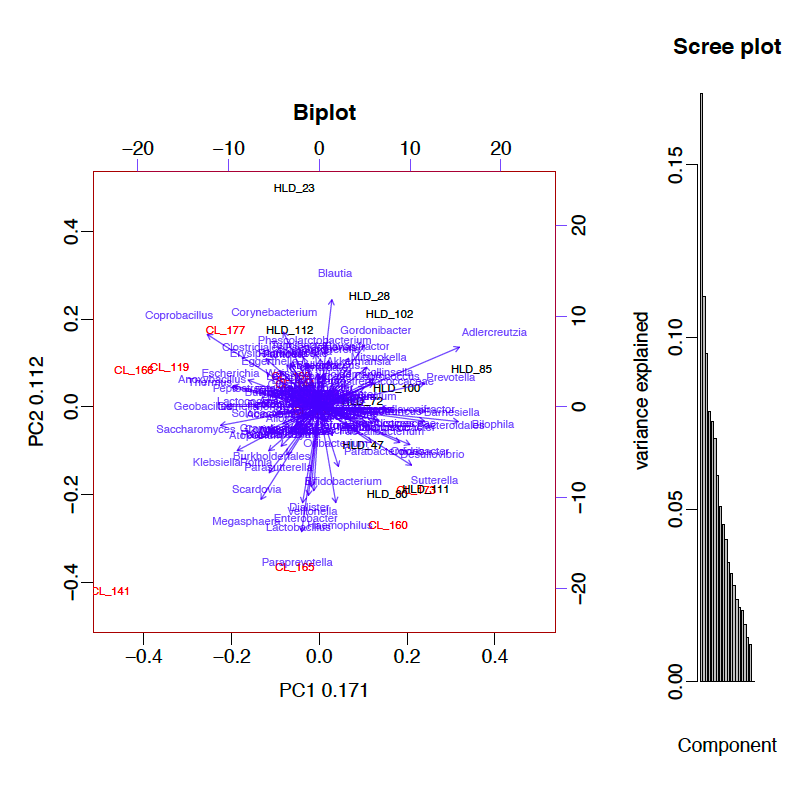
\includegraphics[width=0.95\textwidth]{metaphlan_biplot.png}
\caption{\textbf{Biplot derived from MetaPhlAn.} This biplot was generated from the count table inferred by MetaPhlAn, with taxa filtered such that only taxa with at least 1\% abundance in any sample was kept. Note that the variance explaiend by the first and the second coordinate is not particularly high, indicating that there is not a clear unidirectional separation between groups. Samples from healthy controls are colored black while samples from patients with NASH are colored red.}
\end{center}
\label{nafld_metaphlan_biplot}
\end{figure}

\begin{figure}[h]
\begin{center}
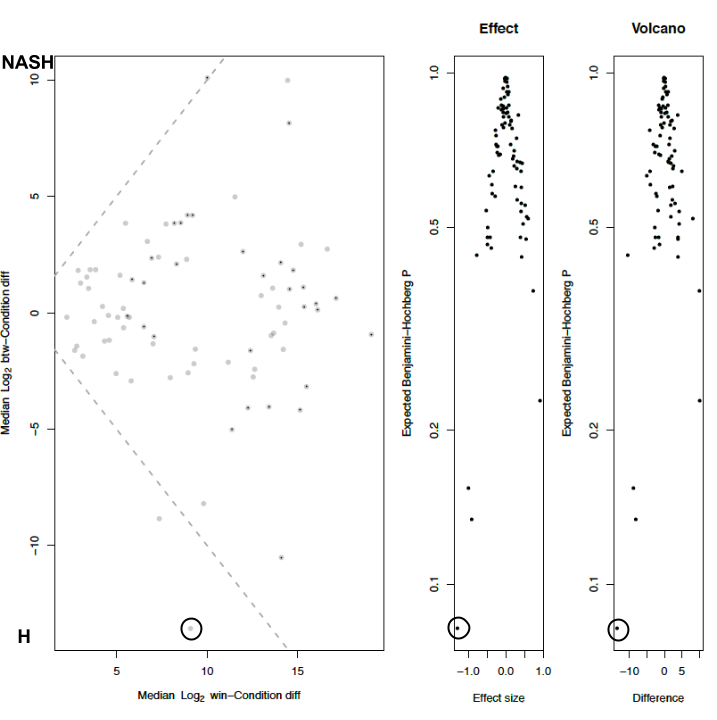
\includegraphics[width=0.95\textwidth]{metaphlan_aldex.png}
\caption{\textbf{Difference within groups vs. difference between groups per taxa, derived from MetaPhlAn.} This plot was generated from the count table inferred by MetaPhlAn, with taxa filtered such that only taxa with at least 1\% abundance in any sample was kept. No taxa are more differential between groups than within groups.}
\end{center}
\label{nafld_metaphlan_aldex}
\end{figure}

\begin{figure}[h]
\begin{center}
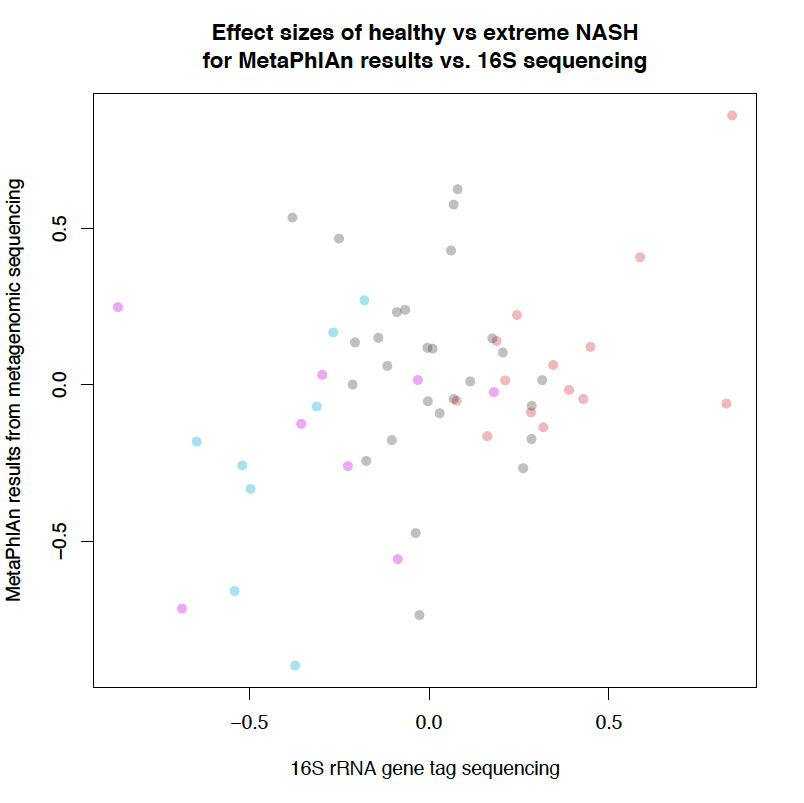
\includegraphics[width=0.95\textwidth]{metaphlan_16s_effects.png}
\caption{\textbf{Effect size correlation between MetaPhlAn and 16S rRNA gene tag sequencing.} For this plot, taxa were amalgamated at the genus level. The Spearman coefficient is 0.5193331. The three samples with identical counts have been removed (otherwise the Spearman coefficent would have been 0.4456304).}
\end{center}
\label{nafld_metaphlan_effect}
\end{figure}

\section{Discussion}

Given the inconsistency in the five papers that have been published about NAFLD and the gut microbiome, we have performed our analysis with care in an effort to find true effects. We found that there was no significant difference between groups by sample clustering (Fig.~\ref{nafld_fig2}) or at the level of the individual OTUs (Fig.~\ref{nafld_fig3}).

There are several factors that would make such a study underpowered. First, the gut microbiome is highly diverse between individuals. This is compounded by the fact that the samples were taken from a diverse Toronto population, including people who immigrated from other countries who likely have different diets. Additionally, the nature of microbiome data is that there are very many more variables (in the form of OTUs or annotated gene functions) than samples.

From Fig.~\ref{nafld_fig4}, the correlation shows that even though there is not enough power to detect a significant difference, the difference from the healthy baseline are moving in the same direction through simple steatosis to nonalcoholic steatohepatitis to extreme NASH.

We hypothesize that there is a characterizable difference in the gut microbiome between patients prone to NASH and healthy controls. Further study with a higher sample size, a more homogenous population, and a greater phenotypic difference between groups may provide the statistical power required to detect the nature of this difference.

\chapter{Discussion}

It is clear that more robust statistical analysis is necessary in this field. The chapter on expanding the UnIFrac toolbox highlighted examples of misuse of unweighted UniFrac in papers published in Cell and Nature. One claimed to find differences in the gut microbiome of mice modelling autism spectrum disorder, compared to healthy controls. The other claimed to find differences in the gut microbiome of humanized mice fed a more traditional fibrous diet compared to mice compared to mice fed a diet similar in composition to the Western diet. These studies had small sample sizes (n = 20 and 10 respectively), used unweighted UniFrac (which we have shown to be unreliable), and had a low amount of variance explained by the principal components axes (14\% on PC1).

The chapter about nonalcoholic fatty liver disease (NAFLD) showcased five studies which all claimed to have found a difference in the gut microbiome of patients with nonalcoholic fatty liver disease compared to healthy controls, but with almost non-overlapping results (Fig.~\ref{nafld_fig1}). Some of the variation can be explained by differences in sequencing platform (Roche 454 vs. Illumina MiSeq). More variation can be explained by the variable region of the 16S rRNA gene chosen for sequencing - one study used V1-2, one study used V3, one study used V4, and the other two studies did not report which variable region was used. Three out of five studies used healthy controls with a lower BMI than the NAFLD group, such that differences due to level of obesity could not be distinguished from differences due to NAFLD. Lastly, only one of the studies performed a multiple test correction, so most of the results could not be distinguished from false positives.

recommendations
- compositional data analysis
- look at your data (variance explained, etc.)
- ways to make inferences on data that are not p-value based (like our effect size stuff)

nature statistics biology

summary/conclusion
- we did some methods development and applied it to nafld
- found that many studies in this field cannot be replicated
- made recommendations

field needs some standards like clinical genomics (other fields?)
GWAS studies - reproducibility/batch effects

microbiome standardized way too early, before they knew what they were looking at
- the human microbiome project
- done by ecologists ?
 — ecological diversity (one of hte HMP paper in supplementary data, found that diversity indices track how deeply you sequence and tell you nothing else)

- learned as they went along, but were under a tight timeline


%% This adds a line for the Bibliography in the Table of Contents.
\addcontentsline{toc}{chapter}{Bibliography}
%% ***   Set the bibliography style.   ***
\bibliographystyle{plain} % (change according to your preference)
%%% ***   Set the bibliography file.   ***
\printbibliography
%% ***   NOTE   ***
%% If you don't use bibliography files, comment out the previous line
%% and use \begin{thebibliography}...\end{thebibliography}.  (In that
%% case, you should probably put the bibliography in a separate file
%% and \include or \input it here).

%Appendices.
\begin{appendices}
\chapter{Workflows}\label{AppA}
\myappendices{Appendix \ref{AppA} \byname{AppA}}
\section{Non-alcoholic fatty liver disease metagenomic workflow}

\subsection{Filter OTUs}
In this experiment, the sequencing depth is expected to have the power to detect a 2 fold change up or down in bacteria that are 0.2\% abundant in a sample. The OTUs were filtered to remove any with an abundance lower than 0.2\% in all samples, and the OTU seed sequences were retrieved.

\subsection{Get reference library genomes}
The list of genomes used in the reference library was created using two sources: the Human Microbiome Project gut reference genomes (http://hmpdacc.org/HMRGD/healthy/), and the NCBI complete and draft bacterial genomes (http://blast.ncbi.nlm.nih.gov/Blast.cgi?PAGE_TYPE=BlastSearch&BLAST_SPEC=MicrobialGenomes).

\paragraph{Human Microbiome Project}\mbox{}\\
The Human Microbiome Project gut reference genomes (http://hmpdacc.org/HMRGD/healthy/) were all added to the reference library genome list for the metagenomic study.

\paragraph{NCBI complete and draft bacterial genomes}\mbox{}\\
The draft and complete bacterial genomes can be queried here: \url{http://blast.ncbi.nlm.nih.gov/Blast.cgi?PAGE_TYPE=BlastSearch&BLAST_SPEC=MicrobialGenomes}. During this process, we ran into a bug using the NCBI webtool and had to search once through the wgs database, and once with Complete Genomes to get both the draft and the complete genomes.

The BLAST output can be downloaded. In this case we were only interested in the genomes that matched with 98\% identity or greater. For these genomes we extracted the GI number, and performed web scraping in Python to visit \url{http://www.ncbi.nlm.nih.gov/nuccore/\<GI number\>} and programatically retrieve the taxon ID. The taxon ID is found in \url{ftp://ftp.ncbi.nlm.nih.gov/genomes/ASSEMBLY_REPORTS/assembly_summary_genbank.txt} and the corresponding FTP link is used to download the genome. For each species found by this method, the genomes for 10 random strains are downloaded (or all of the strains if there are less than 10), to increase the coverage of the library.

\subsection{Get reference library coding sequences}
Some of the genomes have a .gff file which includes the locations of the coding sequences already. For the rest, we used Glimmer \cite{delcher2007identifying} to predict open reading frames.

\subsection{Annotate reference library coding sequences}
Annotation was performed by querying the SEED database \cite{overbeek2005subsystems} using command line BLAST (\url{http://www.ncbi.nlm.nih.gov/books/NBK279690/}). This is the most computationally intensive part of the process and can take a number of days, depending on your computing platform. The specific SEED database we used was downloaded June 2013, and had the fig.pegs from the 2010 SEED database which are missing from the 2013 database manually added in.

\subsection{Map seqeunced reads to reference library}
Once the sequenced reads are available, they can be mapped to the reference library using Bowtie2 \cite{langmead2012fast}. Custom scripts were used to convert the mapping output to a table of counts per annotation per sample, which can then be analyzed with differential expression tools such as ALDEx2 \cite{fernandes2014unifying}.

All of the scripts used to perform the above for the metagenomic non-alcoholic fatty liver disease experiment can be found at \url{https://github.com/ruthgrace/make_functional_mapping_library} in their unedited glory.
\chapter{NAFLD study data collection}\label{AppB}
\myappendices{Appendix ~\ref{AppB} ~\nameref{AppB}}

\subsection{Study Participants}
This cross-sectional study includes 39 NAFLD patients (15 SS, 24 NASH) from the University Health Network (UHN) outpatient liver clinics and 30 healthy living liver donors as healthy controls (HC) from the UHN Liver Transplant Clinic. Patient recruitment occurred from July 2010 to May 2014. The University Health Network and University of Toronto Research Ethics Boards approved this research. All subjects provided their informed written consent.

Patients suspected of having NAFLD due to persistently elevated liver enzymes after ruling out other causes were recruited at their hepatologist appointment prior to liver biopsy. Following a detailed explanation of the study and consent form, and answering of any questions, informed consent was obtained. Eligibility to participate in the study was then considered. For NAFLD patients the inclusion criteria were: a biopsy proven diagnosis of NAFLD (determined during the study), age greater than or equal to18 years, alcohol consumption of less than 20g per day. NAFLD patients were excluded from the study if they had a diagnosis of any other liver disease or HIV infection, if liver transplant was expected to be required within one year, if they had significant liver complications (e.g. variceal bleeding, jaundice, etc.) or any contraindications for liver biopsy, if they were pregnant or lactating, if they had any gastrointestinal disease, or if they were taking any medications known to cause steatohepititis, insulin, NSAIDS, antibiotics, prebiotics, probiotics, or experimental drugs within the last three months. Healthy living liver donors were approached at their first screening appointment for liver donation. Upon completion of informed consent healthy donors were screened for research eligibility. Inclusion and exclusion criteria were the same with the additional inclusion criteria that they must be eligible for live liver donation.

\subsection{Study Visits}
Each participant attended three study visits as outlined in Figure 1. For NAFLD patients, after informed consent was obtained, they were provided with detailed instructions for the completion of a 7-day food record, 7-day activity record, and environmental questionnaire (see below for further details). Patients were also provided with instructions for the collection and transport of their stool sample, which they were requested to return on the day of their scheduled liver biopsy. Usual clinic blood work was also collected at this initial visit for general markers of liver health. On their second visit fasting study-specific blood work was collected and anthropometric measurements were completed. The third visit was the day of their liver biopsy when patients also returned their stool sample and food and activity logs. Healthy living liver donors followed a similar schedule, however, stool samples were typically collected on visit two and the liver biopsy was taken intraoperatively. For further details on all study measurements and processing see below.

\subsection{Clinical Data, Environmental Questionnaire, and Anthropometric Measurements}
Clinical data was collected on study visit one. Study participant’s smoking and alcohol consumption history and medication and supplement use were reviewed, including medications taken in the last three months. Study participants were also asked to answer a number of questions regarding their personal and family history of disease. Age, ethnicity, and menstrual history were also recorded.

An environmental questionnaire was completed and returned with the stool sample. This questionnaire collected information that may affect an individual’s IM composition including country of origin, method of birth (vaginal versus caesarian section), whether they were breastfed as an infant, what kind of pets they have at home, and others.

Anthropometric measurements including height (ht), weight (wt), waist circumference (WC), hipcircumference, and weight-to-hip ratio (WHR) were measured by a trained research professional. Weight was measured using a calibrated hospital-grade chair scale; height was measured using a standometer. Waist circumference was measured at the umbilicus level and hip circumference was measured at the widest point over the buttock. All measurements were taken in triplicate and the average value was used.

\subsection{Nutrition and Activity Assessment}
Each participant was given a food record and activity log to complete in the weekprior to returning their stool sample. Detailed instructions were provided for the completion of both of these tools. The food log included all food and beverages consumed each 24 hours for seven days. In cases where time was insufficient a three-day food record including one weekend day was completed.  Participants used the 2D Food Portion Visual Chart (Nutrition Consulting Enterprises, Framingham, MA) to estimate portion sizes. This is a validated tool which has been used in our previous studies [59, 187, 188]. Food records were reviewed by an experienced registered dietitian and were analyzed using Food Processor Diet and Nutrition Analysis Software (Version 7, ESHA Research, Salem, OR).

Physical activity logs were recorded for 7 days concurrent with the food records. Participants were asked to record any activity, including household chores, the duration of the activity, and the intensity level. Detailed instructions were provided including examples for each intensity level (mild, moderate, strenuous, and very strenuous).  This information was used to calculate daily physical activity units: 1 unit = 30 minutes mild, 20 minutes moderate, 10 minutes strenuous, or 5 minutes very strenuous activity. This is a validated method for measuring physical activity level [189]. Basal metabolic rate (BMR) was calculated using the Harris-Benedict equation: BMR for men = 66.5 + [13.75 × wt(kg)] + [5.003 × ht(cm)] – [6.755 × age(y)], BMR for women = 655.1 [9.563  × wt(kg)] + [1.850  × ht(cm)] – [4.676  × age(y)]. Estimated energy expenditure (EER) was calculated using Health Canada Guidelines: EER for men = 662 – [9.53 x age(y)] + PA x {[15.91 x wt(kg])] + [539.6 x ht(m)]}, and EER for women = 354 – [6.91 x age(y)] + PA x {[9.36 x wt(kg)] + (726 x ht(m)]} where PA is the physical activity coefficients.

\subsection{Biochemistry}
Routine and study specific blood work was drawn after a 12 hour overnight fast on study visittwo. Liver markers were drawn as a routine clinical measure and included: aspartate transaminase (AST), alanine transaminase (ALT), alkaline phosphatase (ALP), and bilirubin. Measures of glucose metabolism included plasma glucose, insulin, hemoglobin A1c (HbA1c), and HOMA-IR which was calculated as fasting glucose (mmol/L) × fasting insulin (mU/L)/22.5 [191]. A lipid profile was also conducted, including total cholesterol, low density lipoprotein (LDL), high density lipoprotein (HDL), and triglycerides (TG). These analyses were conducted by the UHN Laboratory Medicine Program. Liver enzymes and lipid profile were measured using the Architect c8000 system (Abbott Laboratories). LDL was calculated from total cholesterol – HDL. Fasting plasma glucose and plasma insulin were measured by the enzymatic hexokinase method and radioimmunoassay, respectively.

\subsection{Serum Metabolites}
Serum metabolites, including choline, ethanol, and TMA, were measured to evaluate potential implications of bacterial metabolism at a systemic level. For the full list of the 41 metabolites measured see Table 4. Serum was drawn in a fasting state using a gel serum separation vacutainer and was immediately placed in an insulated container with cooling elements. Blood was separated by centrifuge at 4°C at 2800 x g for 20 minutes.  Serum was then aliquoted and stored at -80°C until all study samples were collected. Serum was then shipped to the Metabolomic Innovation Centre (Edmonton, AB) were metabolites were analyzed using nuclear magnetic resonance  spectrometry (NMR), a method which this centre has perfected [192]. The following methods were used by the centre and are stated in their own words [192]: All serum samples were deproteinized using ultrafiltration.  Prior to filtration, two 0.5 mL, 3 KDa cut-off centrifugal filter units (Millipore Microcon YM-3) were rinsed four times each with 0.5 mL of water, then centrifuged at 11 000 rpm for 1 hour, to remove residual glycerol bound to the filter membranes. Two 150 μL aliquots of each serum sample were then transferred into the two centrifuge filter devices. The samples were then spun at a rate of 11 000 rpm for 140 minutes, to remove macromolecules (primarily proteins and lipoproteins) from the sample. The subsequent filtrates were then checked visually for a red tint, which indicates that the membrane was compromised. For those “membrane compromised” samples, we repeated the filtration process with a different filter and inspected the filtrate again.  We then pooled the filtrates that passed the inspections and recorded the volume. If the total volume of the sample was under 300 μL, we added an appropriate amount from a 50 mM NaH2PO4 buffer (pH 7) to the sample until the total volume was 300 μL.  Subsequently, 35 μL of D2O and 15 μL of a standard buffer solution [11.667 mM DSS (disodium-2,2-dimethyl-2-silapentane-5-sulphonate), 730 mM imidazole, and 0.47\% NaN3 in H2O] was added to the sample. The serum sample (350 μL) was then transferred to a standard Shigemi microcell NMR tube for subsequent spectral analysis.

All 1H-NMR spectra were collected on a 500 MHz Inova (Varian Inc., Palo Alto, CA) spectrometer equipped with either a 5 mm HCN Z-gradient pulsed-field gradient (PFG) room-temperature probe or a Z-gradient PFG Varian cold-probe. 1H-NMR spectra were acquired at 25°C using the first transient of the tnnoesy-presaturation pulse sequence, which was chosen for its high degree of quantitative accuracy [193]. Spectra were collected with 128 transients and 8 steady-state scans using a 4 second acquisition time and a 1 second recycle delay.

All FIDs were zero-filled to 64k data points and subjected to line broadening of 0.5 Hz. The singlet produced by a known quantity the DSS methyl groups was used as an internal standard for chemical shift referencing (set to 0 ppm) and for quantification. All 1H-NMR spectra were processed and analyzed using the Chenomx NMR Suite Professional software package version 6.0 (Chenomx Inc., Edmonton, AB), as previously described [194].  Each spectrum was processed and analyzed by at least two experienced NMR spectroscopists to minimize compound mis-identification and mis-quantification.

Serum trimethylamine N-oxide (TMAO) was not detectable using NMR therefore TMAO was measuring using TMAO using a targeted quantitative metabolomics approach by Liquid Chromatography Mass Spectrometry (LCMS). Isotopically-labeled internal standards were added to the serum to facilitate metabolite quantification. Sample extraction was performed on a 96 well plate with a 0.2 µm solvent filter. 10 µL of serum was spiked with the internal standard (TMAO D9) and then 150 µL of methanol with 10 mM ammonium acetate was added for extraction. The plate was shaken for 10 min and centrifuged at 500 rpm for 5 minutes at 4 ºC. Each sample was diluted with 150 μL of water. Seven calibrant solutions with known concentrations went through the same extraction steps. LCMS analysis was performed on AB SCIEX 4000 QTrap mass spectrometer with Agilent 1100 HPLC. 10 µL of the extracted samples were injected onto the Kinetex C18 (2.6 µm, 3.0x100mm, 100A) Column with guard column. Isobaric elution was performed with 90\% A (10 mM ammonium formate in water, PH3) and 10\% B (10 mM ammonium formate in 90:10 Acetonitrile:water, PH3). Total LC method run time was 3 min with flowrate of 500 µl/min. A seven-point calibration curve was generated to quantify the concentration of TMAO in samples.

\subsection{Liver Histology}
Liver biopsies were taken percutaneously (needle biopsy) for NAFLD patients and intraoperatively (wedge biopsy) for HC and preserved immediately in formalin. Liver biopsies were assessed by the same pathologist using standard stains for the diagnosis of NAFLD, morphologic evaluation, and to rule out any iron overload. The evaluation of NAFLD related measures of steatosis, inflammation, and fibrosis were conducted using the validated and reproducible Brunt system. Disease severity was also evaluated using the NAFLD Activity Score (NAS) which accounts for degree of steatosis, lobular inflammation, and hepatocellular ballooning for a final score of 0-8.

\subsection{Stool Sample Collection and Analysis}
On study visit one participants received a stool collection kit, including a plastic collection/storage container with a tightly closing lid, an insulated bag, and cooling elements. Within 24 hours of their next appointment they collected one stool sample, which was frozen immediately after defecation in the patient’s home freezer (-20°C). Participants brought the frozen sample in the insulated bag with cooling elements to their appointment at the hospital, where it will stored at -80C until homogenization.

\subsection{Stool Homogenization}
Stool samples were homogenized prior to DNA extraction for IM sequencing and metabolitemeasurements. The entire sample was first transferred into a sterile masticator bag. The sample was allowed to thaw until a smooth consistency was reached, typically 2-3 hours depending on sample size. Once thawed excess air was released from the bag and the sample was homogenized for two minutes using a masticator blender (IUL, S.A., Barcelona, Spain). This was followed by one minute of hand mastication of any areas that were missed. The corner of the masticator bag was then cut and the sample was aliquoted: 1-2 g samples were stored for metabolite analysis and 0.1-0.2 g aliquots were stored for DNA extraction. Samples were immediately placed on dry ice and then transferred to -80°C for storage until analysis. Weight was recorded for each aliquot and pH was measured for each sample.

\subsection{DNA Extraction}
DNA was extracted using the E.Z.N.A. Stool DNA Kit (Omega Bio-Tek, Norcross, GA) and amodified manufacturer’s protocol. Briefly, 200 mg of glass beads and 600 µL of SLB buffer were added to the sample and vortexed at maximum speed for 15 minutes. 20 µL of lysozyme (20mg/ µL) was added and flicked to mix then incubated at 37°C for 30 minutes. 60 µL DS Buffer and 20 µL Proteinase K were added and vortexed to mix then incubated at 70°C, 300 rpm, for 13 min, vortexing at T=6.5 minutes and T=13 minutes. The incubation temperature was then increased to 95°C for an additional 5 minutes. 200 µL SP2 Buffer was added and mixed by vortex for 30 seconds then put on ice for 5 minutes. The mixture was then centrifuged at 21 000 rcf for 7 minutes and the supernatant was transferred to a new 1.5 mL centrifuge tube while the old tube was discarded. 200 µL HTR Reagent was added and vortexed at maximum speed for 10 seconds, then incubated at room temperature for two minutes and centrifuged for an additional two minutes. The supernatant was again transferred to a new 1.5 mL centrifuge tube and the addition of HTR Reagent and following steps were repeated once. After transfer to the last 1.5 mL tube 250 µL of BL buffer and absolute ethanol were added and vortexed for 10 seconds.

The DNA column was placed into a collection tube and 100 µL of 3M NAOH was added. This was incubated for four minutes and centrifuged for one minute. 100 µL of distilled water was added to the DNA column and centrifuged for one minute. 800 µL of sample was transferred into the DNA column and centrifuged for one minute. The contents of collection tube was discarded and the remainder of the sample was transferred into the DNA column and again centrifuged for one minutes. The flow-through and collection tube were discarded. The column was then placed into a new 2 mL collection tube and 500 µL of VHB Buffer was added to the column. This was centrifuged for 30 seconds and the flow-through was discarded. 700 µL of DNA Wash Buffer was then added to the DNA column and centrifuged for one minute and the flow-through and tube was discarded. This washing stage was repeated once. The column was then transferred to a new 2 mL collection tube, centrifuged for one minute and the flow-through was discarded. The tube was then centrifuged again for two minute, this time with the cap open, to the dry the column. The column was finally transferred to a new 1.5 mL tube, 100 uL of distilled water was added, this was incubated for five minutes, centrifuged for two minutes, the column was removed and then the final DNA sample was analyzed for purity and concentration using the Nanodrop 1000 Spectrophotometer (ThermoScientific, Rockford, IL). DNA samples were stored at -80°C.

\end{appendices}

%CV only relevant stuff... not full CV.
\addcontentsline{toc}{chapter}{Curriculum Vitae}
\chapter*{Curriculum Vitae}
\begin{table}[ht]
\begin{tabular}{ll}
\textbf{Name:} & \firstname{} \lastname\\\\
\textbf{Post-Secondary} & The University of Western Ontario\\
\textbf{Education and}& London, ON\\
\textbf{Degrees:}& 2010-2014 B.M.Sc.\\\\
& University of Western Ontario\\
& London, ON\\
& 2014-2016 M.Sc.\\\\
\textbf{Honours and}& Western Gold Medal\\
\textbf{Awards:}& 2014\\\\
& Leland Ritcey Prize\\
& 2011\\\\
\textbf{Related Work}& Summer Intern, Persistent Disk Team\\
\textbf{Experience:}& Google Inc., New York office\\
& Summer 2015\\\\
& Google Summer of Code Participant\\
& Bader Lab, University of Toronto\\
& Summer 2014\\
\end{tabular}
\end{table}
\subsubsection*{Publications:}
Wong, Ruth G., Jia R. Wu, Gregory B. Gloor. "Expanding the UniFrac toolbox." Submitted to PLOS ONE.
\end{document}

